% ****** Start of file apssamp.tex ******
%
%   This file is part of the APS files in the REVTeX 4.2 distribution.
%   Version 4.2a of REVTeX, December 2014
%
%   Copyright (c) 2014 The American Physical Society.
%
%   See the REVTeX 4 README file for restrictions and more information.
%
% TeX'ing this file requires that you have AMS-LaTeX 2.0 installed
% as well as the rest of the prerequisites for REVTeX 4.2
%
% See the REVTeX 4 README file
% It also requires running BibTeX. The commands are as follows:
%
%  1)  latex apssamp.tex
%  2)  bibtex apssamp
%  3)  latex apssamp.tex
%  4)  latex apssamp.tex
%
\documentclass[%
 reprint,
%superscriptaddress,
%groupedaddress,
%unsortedaddress,
%runinaddress,
%frontmatterverbose, 
%preprint,
%preprintnumbers,
%nofootinbib,
%nobibnotes,
%bibnotes,
 amsmath,amssymb,
 aps,
%pra,
prb,
%rmp,
%prstab,
%prstper,
floatfix,
]{revtex4-2}

\usepackage{graphicx}% Include figure files
\usepackage{dcolumn}% Align table columns on decimal point
\usepackage{bm}% bold math
\usepackage{hyperref}% add hypertext capabilities
\hypersetup{colorlinks=true,urlcolor={blue},citecolor={blue}, linkcolor={blue}}
\usepackage{amsmath} % or simply amstext
%\newcommand{\angstrom}{\textup{\angstrom}}
\usepackage{siunitx}
\usepackage{color}
\usepackage[normalem]{ulem}
\usepackage{diagbox}
\usepackage{import}
\usepackage{multirow}
\usepackage{xr} % referencing across multiple files
\usepackage{cleveref} % cite figures in SI
\usepackage[dvipsnames]{xcolor}

%\usepackage{url}            % simple URL typesetting
%\usepackage[mathlines]{lineno}% Enable numbering of text and display math
%\linenumbers\relax % Commence numbering lines
%\usepackage{nameref}

%\usepackage[showframe,%Uncomment any one of the following lines to test 
%%scale=0.7, marginratio={1:1, 2:3}, ignoreall,% default settings
%%text={7in,10in},centering,
%%margin=1.5in,
%%total={6.5in,8.75in}, top=1.2in, left=0.9in, includefoot,
%%height=10in,a5paper,hmargin={3cm,0.8in},
%]{geometry}

%RZK: do not edit red text
\newcommand{\lock}{\color{red}}
\newcommand{\comm}{\color{Purple}} %comment
\newcommand{\sinfo}{Supplementary Information}

% Use Supp Info labels with SI- prefix
\externaldocument[SI-]{SI}

\begin{document}

\title{Adatoms in the surface Ullmann coupling}

\author{Zhenzhe Zhang}
\author{Dmitrii F. Perepichka}%
\email{dmitrii.perepichka@mcgill.ca}
\author{Rustam Z. Khaliullin}
\email{rustam.khaliullin@mcgill.ca}
\affiliation{%
 Department of Chemistry, McGill University, 801 Sherbrooke St West, Montreal, QC H3A 0B8, Canada
}%

%\date{\today}% It is always \today, today,
             %  but any date may be explicitly specified

\begin{abstract}
There is a mounting evidence from experimental and modeling studies that metal atoms can be raised above or completely extracted from a metal surface during the Ullmann reaction. 
This manuscript reviews the results of experimental and computational studies of the surface Ullmann coupling that shed light on the role of surface adatoms in its mechanism. A particular focus is on the early stages of the polymerization and coupling of two monomers.
\end{abstract}

\maketitle

%\tableofcontents

%RZK. What a variety of labels mean. 
%RYK - to be replaced with the actual value later
%R1111 or RZKmmdd - mm denotes month, dd - denotes day
%RZKX - these are low priority comments, which will be promoted to regular labels later 
%RZZK - ignore! These labels keep track of my own revision process

%%% GENERAL REMARKS %%%

%RZK: Detailed description of the figure. Take a look at the original publication. Reprinted from~\cite{RZK} with permission of American Chemical Society or PUBLISHER. See the LaTeX comment below. If you take a figure from a publication it is very important to cite the work and obtain publisher's permission. We need to make sure that all our borrowed figures satisfy copyright permissions. For example, see: https://www.stm-assoc.org/2016_01_05_Guidelines_for_Quotation_From_Journal_Articles.pdf


Color-coding: 

{\lock RZK and ZZ contributed and agree.}

{\comm Some in-line comments by RZK.}

\textcolor{blue}{Written by ZZ, to be reviewed by RZK.}

{Unclassified text.}

Zhenzhe, if you edit the red text, please save the original as a LaTeX comment. I often need to revert your changes and it takes too much time.

\section{Introduction}

%RZK0423: The detailed review of the classical Ullmann reaction is saved in the branch named Review-Intro. Dima's comments from January 2021 have not been fully incorporated into the saved version.

\subsection{On-surface Ullmann coupling}

{\lock

%RZZK: Dima's comment: ``Discuss GNRs and 2D polymers, give some key figures - to tell the reader why they should care to read the rest of the paper.'' I think figures will be useful in the thesis but not in the research article.

Unique and tunable properties of $\pi$-conjugated organic polymers such as one-dimensional (1D) graphene nanoribbons~\cite{ullmann_106, ullmann_45, ullmann_107, ullmann_101}
%RZK0506: avoid mentioning materials that are not relevant for this review.
%, hexagonal boron-nitride~\cite{ullmann_110, ullmann_111, ullmann_112} 
and two-dimensional (2D) [layered] covalent organic frameworks {\comm [RZK0506: check whether the references are suitable for 2D $\pi$-conjugated COFs~
\cite{ullmann_108, ullmann_109}]} make them promising candidates to produce a variety of electronic and optoelectronic devices~\cite{ullmann_113, ullmann_114}.
%
The utilization/application of these materials requires scalable methods to fabricate/produce/synthesize extended polymer structures with low defect density.
%{\comm RZK0506: Should we mention the challenge of decoupling the polymer from the metallic surface to make semiconducting devices. }%end comm
%
%RZK0506: On-surface polymerization is a rapid-developing field aimed at achieving the constructions of unprecedented 1D or 2D polymers with novel structures and revolutionary properties\cite{ullmann_105, ullmann_33, ullmann_70}. 
The on-surface Ullmann reaction is currently viewed as a promising bottom-up strategy to assemble, in mild conditions, atomically precise $\pi$-conjugated organic polymers with high degree of control over their electronic properties~\cite{ullmann_33}. 
%
%A recent surge of interest in electronic devices based on low-dimensional organic nanostructures with $\pi$-conjugated backbones has led to a renewed attention to the Ullmann process.
%The recent surge of interest in bottom-up fabrication of functional nanostructures on surfaces....
%
The on-surface Ullmann reaction has been developed from its classical version -- nucleophilic substitution reaction between aromatic halides that proceed in solution in the presence of metallic copper leading to the formation of a carbon-carbon bond. 
Since its discovery in 1901~\cite{ullmann_01}, the classical Ullmann coupling has rapidly become one of the key reactions in organic synthesis with its scope extended to multiple reactants and Cu-containing catalysts~\cite{ullmann_29,ullmann_30,ullmann_31,ullmann_32, ullmann_115, ullmann_116, ullmann_117, ullmann_118, ullmann_119, ullmann_120, ullmann_121, ullmann_122}.
The well-established ability of the Ullmann reaction to create bonds between aromatic carbon atoms thus coupling their $\pi$ systems has been adapted to perform synthesis on metal surfaces, which serve as both a low-dimensional confining template and catalyst.
In the context of surface reactions, the term Ullmann coupling has been extended to refer to the reaction on a variety of metals, most often copper, silver and gold.

One of the first fundamental studies of the surface-confined coupling of iodobenzene to biphenyl under ultrahigh vacuum condition was reported by Bent~\textit{et al.}~\cite{sur_sci01} in 1992. with a series of pioneer and extended exploration\cite{ullmann_127, ullmann_128, ullmann_129, ullmann_87}.
%
The intermediate species of this reaction were inspected using STM imaging by Weiss \textit{et al.} in 1998~\cite{langm01}. 
In 2004, it was demonstrated that linear \emph{protopolymers}---aligned monomer units that have not yet reacted to form the final polymer---could be obtained by depositing \textit{para}-diiodobenzene on Cu(111) at 77 K~\cite{jacs01}. 
%
%This insight showed that the Ullmann coupling can be used not only to synthesize organic molecules but periodic polymers as well. 
These protopolymers have later been identified by Lipton-Duffin \textit{et al.} as periodic organometallic intermediates linked \textit{via} carbon-metal-carbon bonds~\cite{ullmann_88}.
%Remarkably, the Ullmann reaction has been employed for the first synthesis of covalently-bonded nanostructures from molecular building blocks on metal surfaces.
And Grill \textit{et al.} have prepared patches of a 2D polymer from \textit{tetrakis}(bromophenyl)porphyrin on the Au(111) surface.
%the coupling between brominated tetraphenyl-porphyrins on the Au(111) surface was performed by Grill \textit{et al.}~\cite{Naturenano2007} in 2007.
%
Since then, surface Ullmann coupling has become one of the most common on-surface polymerization methods. It has been utilized to create covalently-linked extended macromolecular structures including ordered polymer wires, atomically precise graphene nanoribbons and organic 2D materials on a variety of metal surfaces starting from halogenated aryl precursors~\cite{ullmann_33,ullmann_34, ullmann_42, ullmann_43, ullmann_45, ullmann_46, ullmann_47, ullmann_48}. 

}

%RZK0506: The following can be re-inserted in the right place.
%The choices of monomer and surface are considered as the main challenge for on-surface polymerization. Highly reactive monomers or surfaces will both promote the decomposition or desorption of monomers in high vacuum reaction condition, on the other hand, inert monomers or surfaces can lead to the desorption upon annealing activation. The issue of chemical reactivity underlines the popularity and practicality of on-surface Ullmann coupling methods.



\subsection{Mechanism of on-surface Ullmann coupling}

{\lock

Although numerous nanostructures have been obtained on metal surfaces via Ullmann coupling, our knowledge of the mechanism of the surface processes still remains incomplete. 
A thorough understanding of the mechanism of on-surface Ullmann reaction is essential for tuning reaction conditions and for rational, more precise design of monomers that produce the polymers that match a chosen metal surface.

%RZK-REVIEW: The focus of the following review of the Ullmann coupling mechanism is entirely on the formation of a carbon-carbon bond from halogen-containing precursors on Cu, Ag and Au surfaces. A particular attention is paid to the monohalogenated benzenes. 

The overall coupling process can be divided into the elementary steps (Fig.~\ref{fig_mecha}) described in detail below. It is widely accepted that aryl halide molecules physisorbed on metal surface lose their halogens forming surface-bound aryl radicals. These intermediates diffuse on the surface and, once sufficiently close to each other, combine with the formation of an organometallic intermediate with a carbon-metal-carbon bridge. This intermediate undergoes reductive elimination to form a covalent carbon-carbon bond between the two aryls. It should be noted that the surface Ullmann coupling proceeds through the formation of the organometallic intermediates similar to those encountered in the reaction in solution (Fig.~\ref{SI-fig:classical} in \sinfo).

\begin{figure*}[tb]
\centering
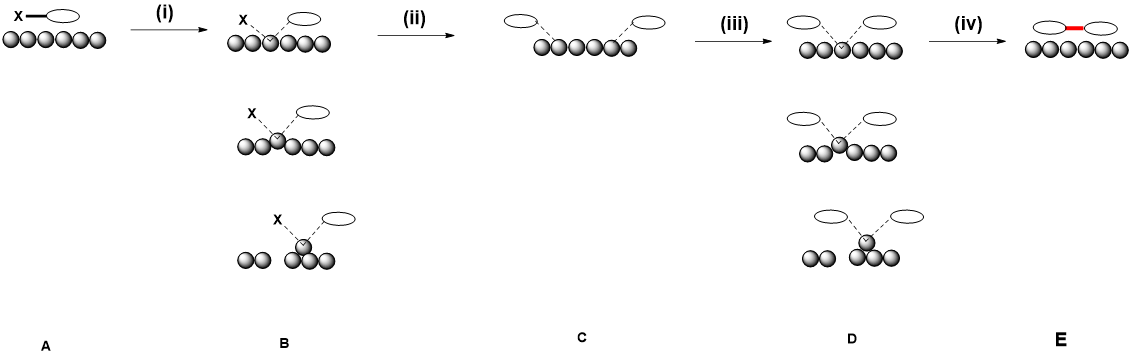
\includegraphics[width=0.9\textwidth]{Fig/mechanism.png}
\caption{Schematic representation of elementary steps of a surface Ullmann coupling process. The following steps are shown: physisorption, dehalogenation, diffusion, formation of the organometallic bridge and then carbon-carbon bond. RZK0422: This figure needs significant improvement or it can be removed altogether. If we decide to keep it, use new pictograms and labels. It is unclear whether the adatom pathway should be shown.}
\label{fig_mecha}
\end{figure*}

}%end lock

\subsubsection{Dehalogenation}

{\lock

The first fundamental step of surface Ullmann coupling is the dissociative dehalogenation of organic precursors adsorbed on the surface. In this step, the carbon-halogen bonds of the precursor are broken whereas the carbon-metal and halogen-metal bonds are formed. 

%RZK0426: Find new place for the sentence below: The thermodynamics and kinetics of the process are primarily determined by the relative strength of the broken and formed bonds. 

}%lock

%RZK0108: This subsection needs more work following the guidelines discussed in December. Trends in experimental data should be presented first, desirably for Ph-X. Your review will be particularly strong if the trends are discussed across all three metals and three halogens for Ph-X. After experiments, discuss if the trends can be reproduced from simple bond-strength models. Then, present a short summary of DFT calculations to say if the experimental trends can be reproduced using electronic structure methods. I only rearranged your text a bit, you must work on it extensively.

%ZZ0223 delete: The following data illuminates the strong influence of surfaces and halogens on the first step of the Ullmann coupling of two Ph-X. For instance, the dissociaton of iodobenzene occurs at \SI{175}{\kelvin} on Cu(111)~\cite{sur_sci01}, \SI{200}{\kelvin} on Ag(111)~\cite{sur_sci02} and \SIrange{200}{250}{\kelvin} on Au (111)~\cite{sur_sci03}.
%The same trend has been observed for bromobenzene with a higher temperature on all surfaces. RZK0122: Find temperatures for bromo and chloro-benzene.
%ZZ: no experiment data to exact bromo- and chlorobenzne)

%RZK0426: You keep using wrong tenses despite my repetitive recommendations to pay attention to this. This is because you do not invest sufficient time to re-read your writing. 

\textcolor{blue}{
The type of halogens and surfaces have been illuminated of strong influence on this first step of the Ullmann coupling of two Ph--X. In experiment, the break of most Ph--X bonds will occur at different temperature based on the halogens and the metal substrates. For instance, the dissociation of iodobenzene will be fulfilled at \SI{175}{\kelvin} on Cu(111)~\cite{sur_sci01}, \SI{200}{\kelvin} on Ag(111)~\cite{sur_sci02} and \SIrange{200}{250}{\kelvin} on Au (111)~\cite{sur_sci03}. 
Theoretical work also proves the same trend of iodobenzene on these three surfaces, additionally bromobenzene also shows the similar tendency. As shown in Fig.~\ref{fig:dehalo}~\cite{jacs2013}, the activation barrier and reaction enthalpy of these two precursors both decrease in the order Au $>$ Ag $>$ Cu based on DFT calculations. This data is consistent with the reaction condition of iodobenzene highest on Au(111) and lowest on Cu(111). Br\o nsted-Evans-Polanyi relation states that the activation energy and the reaction enthalpy are linearly dependent. The activation energy for this exothermic dehalogenation of bromobenzene and iodobenzene on (111) metal surfaces are calculated to be \SIrange{0.4}{1.0}{\electronvolt}. And the barrier of iodobenzene keeps around \SI{0.3}{\electronvolt} lower than bromobenzene for all surfaces. This decline can be explained by the dissociation energy of a C--I bond being $\sim$\SI{0.65}{\electronvolt} lower than that of a C--Br bond~\cite{Arpc1982}. The reaction enthalpy of deiodination is also lower than debromination by \SIrange{0.1}{0.4}{\electronvolt}.}
%RZK0123: Any data on chlorobenzene? (ZZ: I did not find for chlorobenzene)


%RZK0122: The following paragraph is taken from your mechanism summary. It should be discussed here instead. 
%ZZ0223 delete: The dehalogenation of other organic precursors follow the same trends observed for Ph-X. it has been observed that the reactivity trend decrease in the order Ar--I $>$ Ar--Br $>$ Ar--Cl both in experiment and theoretically~\cite{ullmann_52}. This also means that the dissociation of Ar--I bond on metal surface requires the lowest temperature. In addition, the energy barrier of dehalogenation is the highest on Au(111) surface, the lowest on Cu(111) surface both in experiment and in theoretical calculations~\cite{jacs2013}. It has also reported that the miller index of metal surface will also influence the reaction energy of dehalogenation~\cite{ullmann_57}. 

{\color{blue}
Dehalogenation of a variety of other precursors have also been reported, not only limited to Ph--X. For 1,4-dihalobenzene molecules on Cu(110) surface, XPS spectra revealed that dechlorination of dichlorobenzene will be completed at temperature above \SI{400}{\kelvin}~\cite{ullmann_52}, while the cleavage of C--Br, C--I bonds of dibromobenzene, diiodobenzene on Cu(110) will finish under room temperature and deiodination is estimated to require a lower temperature than debromination. Similar trend as Ph--X on difference surface also show for other presursors. The onset temperature for debromination of 1,3,5-tris(4-bromophenyl)benzene on Ag(111) is \SI{75}{\kelvin} lower than on Au(111), and on Au(111) surface the temperature need to be above \SI{325}{\kelvin}. In addition, the molecule hexaiodo-substituted macrocycle cyclohexa-m-phenylene is demonstrated to complete dehalogenation on Cu(111), Ag(111) and Au(111) surface all at room temperature~\cite{ullmann_65}, which indicates that the size of molecule and the quantity of halogens on molecule also possess effect on the dehalogenation conditions.

Dehalogenation on surface are influenced by various factors, such as halogen types and quantities, precursor size as well as the surfaces. The role of halogens and surfaces are well-documented up till now. It can be summarized as the trend of dehalogenation energy follows the order Ar--Cl $>$ Ar--Br $>$ Ar--I for halogen types and Au $>$ Ag $>$ Cu for surfaces.
}

%ZZ0223 delete: To explain the observed differences in reactivity, the following trends in the bond strength have been derived from model molecular systems.
%
%\begin{eqnarray}
%\begin{split}
%\text{C--Cl} > \text{C--Br} > \text{C--I} \\ 
%\text{Cu--C} > \text{Au--C} > \text{Ag--C} \\
%\text{Cu--Cl} > \text{Cu--Br} > \text{Cu--I}\\
%\text{Ag--Cl} \approx \text{Ag--Br} > \text{Ag--I} \\
%\text{Au--Cl} > \text{Au--I} > \text{Au--Br}
%\end{split}
%\end{eqnarray}
%
%ZZ0223 delete: The bond dissociation energy of diatomic and CX$_4$ molecules have been used in the cases of the metal-halogen bonds~\cite{ullmann_62} and carbon-halogen bonds~\cite{ullmann_63}, respectively. The relative strength of metal-carbon bond strength has been estimated using the metal-carbon bond distances in M-(CH$_3$)$_2$ molecules~\cite{ullmann_61}.

%ZZ0223 delete: By combining the strength of all metal-halogen bonds shown above the following series emerges
%
%\begin{gather*}
%\text{Cu--Cl} > \text{Cu--Br} > \text{Au--Cl} \approx \text{Au--I} \approx %\text{Ag--Br} \approx \\
% \approx \text{Ag--Cl} > \text{Ag--I} > \text{Au--Br} > \text{Cu--I}
%\end{gather*}
%

RZK0108: Why you are ordering the strength of metal-halogen bonds? Is it uselful for predicting of the kinetics of the first step (i.e. reaction temperature)? I do not expect this trend to be suitable for the thermodynamics that is certainly affected not only by M-X strength but also by C-X and C-M strengths. We need to predict the energy of this step: C-X bond is broken, C-M bond is formed, X-M bond is formed. Has it been done in any review articles?

%ZZ0223 delete: DFT calculations have estimated the activation barrier for the exothermic dehalogenation of bromobenzene and iodobenzene on (111) metal surfaces to be \SIrange{0.4}{1.0}{\electronvolt}~\cite{jacs2013}. As shown in Fig.~\ref{fig:dehalo}, the activation barrier and reaction energy decrease in the order Au $>$ Ag $>$ Cu and are \SIrange{0.1}{0.5}{\electronvolt} lower for iodobenzene than bromobenzene. The latter is due to the dissociation energy of a C--I bond being $\sim$\SI{0.65}{\electronvolt} lower than that of a C--Br bond~\cite{Arpc1982}. RZK0123: Any data on chlorobenzene?

\begin{figure}[tbh]
\centering
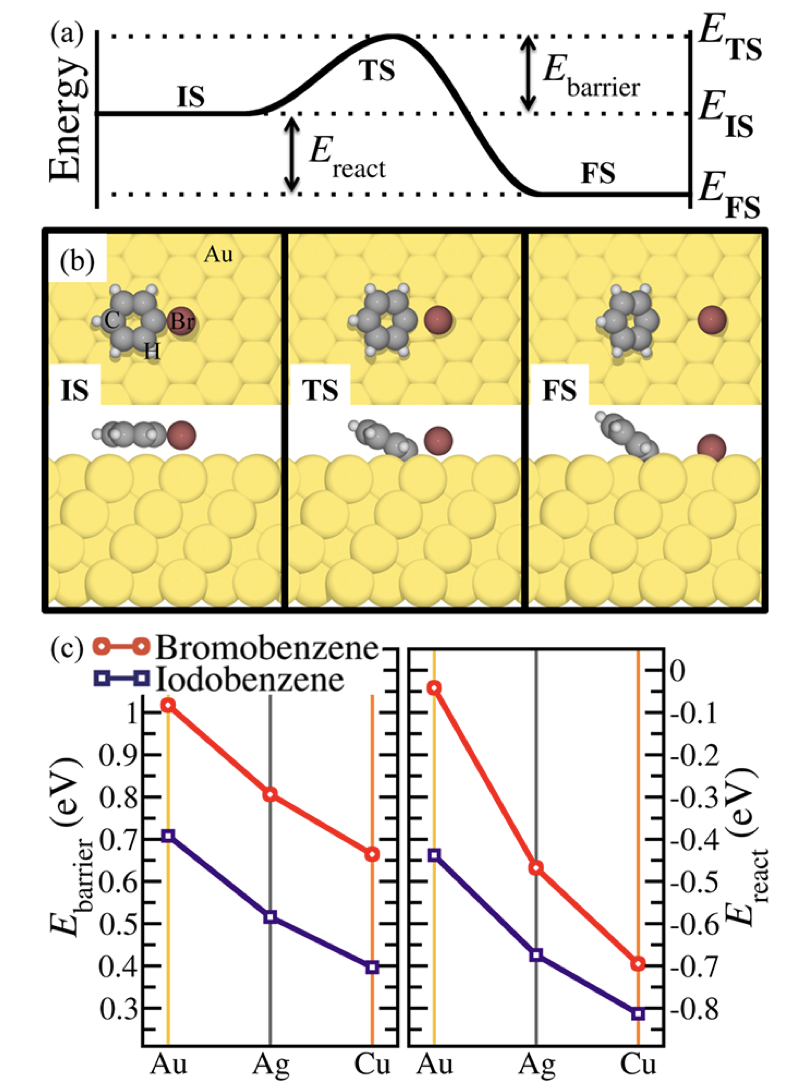
\includegraphics[width=0.75\columnwidth]{Fig/dehalogentaion.png}
\caption{(a) Definitions of the energy barrier and reaction energy for dehalogenation reactions. (b) The dissociation of bromobenzene on Au(111), depicting top and side views of the initial state (IS), transition state (TS), and final state (FS) of the reaction. (c) Energy barrier (left) and reaction energy (right) for the dissociation of bromobenzene and iodobenzene on the (111) facets of Au, Ag, and Cu. Adapted from Ref.~\cite{jacs2013}} 
\label{fig:dehalo}
\end{figure}

\subsubsection{Diffusion}

{\lock

The dehalogenation step produces organometallic intermediates with carbon atoms covalently bonded directly to metal atoms. 
The diffusion of these species, which has been observed experimentally and studied computationally, plays a decisive role in the further coupling process. 
A high mobility of molecules increases the chances of two molecules moving closer to each and forming a bond. Therefore, low energy barriers for diffusion process are a prerequisite for the self-assembly of well-ordered networks.

Among dehalogenated precursors, the diffusion of a phenyl group has been studied most thoroughly. 
Computational studies have considered sliding or flipping mechanisms of diffusion. 
In the sliding diffusion, a phenyl group keeps its orientation to the surface in the initial, transition and final states. The energy barrier of the sliding diffusion on (111)metal surfaces decreases from \SI{0.44}{\electronvolt} on Cu to \SI{0.29}{\electronvolt} on Ag and to \SI{0.22}{\electronvolt} on Au~\cite{jacs2013}. 
In the flipping diffusion, a phenyl group increases its tilting angle, achieves the upright configuration and then overturns to bind to an adjacent metal atom. 
For this diffusion mechanism, the change in the magnitude of the diffusion barriers follows a different trend and decreases from \SI{0.19}{\electronvolt} on Au to \SI{0.07}{\electronvolt} on Cu and to \SI{0.06}{\electronvolt} on Ag~\cite{pccp2010, jacs2013}. 
The low calculated barriers agree with STM studies that have revealed that dehalogenated phenyl groups diffuse on the Cu (111) surface at temperatures as low as \SI{77}{\kelvin}~\cite{langm01}.

It should be noted that the flipping mechanism may not contribute significantly to the diffusion of large precursor molecules, especially those anchored to the surface by several covalent bonds. The stronger surface-molecule interaction will favor diffusion mechanism with the molecular plane remaining parallel to the surface. 
For example, dehalogenated cyclohexa-\textit{m}-phenylene diffusing on copper and silver remains parallel to the surface ~\cite{RZK0426:reference-is-needed}. %RZZK: Is the reason clear? ``because of the multiple covalent bonds with metal atoms and stong interactions between its $\pi$-electrons and metal atoms.''
In addition, the diffusion is often affected by the nature of the substrate. For cyclohexa-\textit{m}-phenylene, the DFT calculated diffusion energy barrier on Cu(111) is \SI{1.4}{\electronvolt} higher than that on Ag(111)~\cite{ullmann_65}. This is due to stronger molecule-surface interactions with copper atoms compared to silver atoms.

Halogen atoms chemisorbed on the surface can also undergo the diffusion process. The binding energy of halogens and their diffusion barriers have been investigated using DFT calculations~\cite{jacs2013}, which show that halogens hop between fcc and hcp hollow sites with the the bridge site being the transition state. The diffusion barriers for a variety of metal-halogen combinations have been found (RZK0426: OR calculated?) to be in the \SIrange{0.02}{0.11}{\eV} range (Table~\ref{table:1}), implying that halogen atoms are highly mobile on the three metal surfaces at relevant temperatures. The barrier is largest on Au(111) and smallest on Cu(111). 
At high surface coverage, halogens atoms bonded to the surface can hinder the diffusion of organic precursors preventing them from approaching each other and hence slowing down the coupling process. 

}

%RZK0426: Dima's comment: "I think we should also disucss diffusion of multifunctional monomers (eg, our JACS2016 and Bieri et al)". Imo, it is relevant only if when we prepare the review manuscript.

\begin{table}[h!]
\centering
\begin{tabular}{ |p{3cm}||p{1.5cm}|p{1.5cm}|p{1.5cm}|  }
 \hline
 \multicolumn{4}{|c|}{Energy barrier of diffusion (\si{\electronvolt}) } \\
 \hline
 Atom     & Cu(111) &Ag(111) & Au(111)\\
 \hline\hline
 Chlorine   &0.08   &      &0.02\\
 Bromine    &0.06   &0.07  &0.09\\
 Iodine     &0.06   &0.06  &0.11\\
 \hline
\end{tabular}
\caption{(RZK0426: Calculated?) Energy barrier of halogens diffusing on different metal surfaces. RZK0426: The origin of this data (experiment, calculations?) is unclear, citation is missing.}
\label{table:1}
\end{table}

\subsubsection{Formation of carbon--metal--carbon intermediates} \label{sec:dimerized}

{\lock

A carbon--metal--carbon (C--M--C) intermediate forms when two molecular fragments diffuse close to each other and become bound to the same metal atom, without yet creating a direct covalent C--C bond. Since the distance between two carbon atoms in such C--M--C bridges is significantly larger than in a covalent bond, their existence has been confirmed in multiple STM and AFM experiments~\cite{jacs2011, ullmann_88}, corroborated with computational studies.

\begin{figure}[ht]
\centering
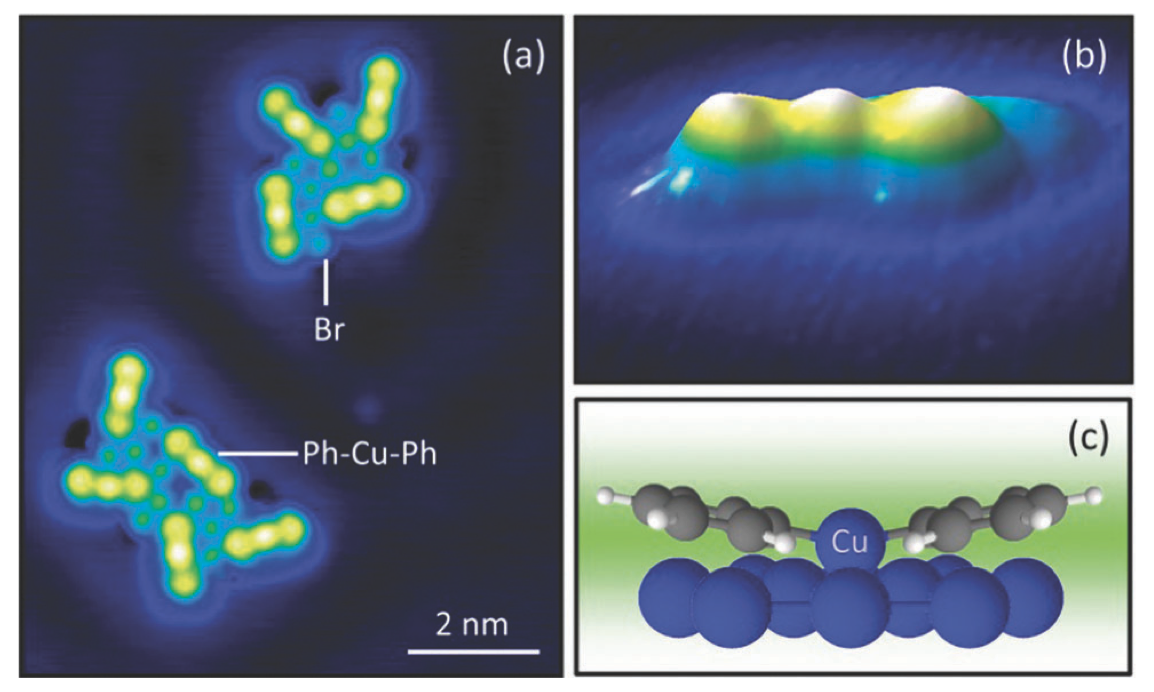
\includegraphics[width=0.85\columnwidth]{Fig/phenylorgano.png}
\caption{STM images and model of the Ph--Cu--Ph organometallic intermediate formed at \SI{160}{\kelvin}. Images are collected at \SI{5}{\kelvin}.  (a) Clusters of the intermediates and Br atoms. (b) 3D rendering of a single phenyl–Cu–phenyl intermediate. (c) Model of two phenyl groups bonded to the Cu atom. Adapted from Ref.~\onlinecite{ullmann_67}.}
\label{fig:organ}
\end{figure}

STM images of phenyl groups on Cu(111) show that structures consisting of two groups bound to the same metal atom form at \SI{160}{\kelvin} (Fig.~\ref{fig:organ}). The measured geometry of these bridge intermediate structures agree with those obtained from DFT modeling~\cite{ullmann_67}. 
Calculations have shown that the formation of Ph--Cu--Ph from two phenyl intermediates attached to two adjacent copper atoms on Cu(111) is barrierless and proceeds with the release of \SI{0.30}{\electronvolt} of energy~\cite{pccp2010}.
%This result is obtained using the dispersion corrected PBE functional with dual Gaussian and plane-wave basis set.
{\comm RZK0426: Dima's comment: ``I would consider giving brief the details of calculations when citing the calc energies - to facilitate comparisons.'' It would be usefull but, if we are to add calculation details, this should be done consistently throughout the introduction, not in just this instance. For now, I will commented out your computational details to keep the description consistent with the rest of the introduction.}

}

{\lock

The existence of organometallic bridges has also been demonstrated for other aryls. Based on a comparative analysis of structures in STM images and geometries from DFT calculations, diiodobenzenes were both proven to form a protopolymer bridge structures at room temperature~\cite{ullmann_88}.
Similar bridge intermediates are formed at room temperature when dibromoterphenyl is deposited on Cu(111) and Ag(111) surfaces~\cite{jacs2011, PCCP2012}.
1,3,5-tris(4-bromophenyl)benzene has also been confirmed to form bridge structures on Cu(111), Ag(110)~\cite{ullmann_89} at room temperature and Au(111) at \SIrange[range-phrase = --]{300}{390}{\kelvin}~\cite{ullmann_90}. 

Although the activation energy of the bridge formation has not been measured directly, it has been inferred, based on an STM analysis of competing elementary steps in the Ullmann coupling of 1,3-bis(p-bromophenyl)-5-(p-iodophenyl)benzene on Ag(111) surface~\cite{ullmann_91}, that the energy barrier of the bridge formation is lower than that of the dehalogenation step. 

}

%It has been established that the rate-determining step on the path toward bridge intermediates is dehalogenation~\cite{ullmann_91}. 

%When 1,3-bis(p-bromophenyl)-5-(p-iodophenyl)benzene is deposited on Ag(111) surface at room temperature, C--M--C intermediates are formed along with the proceeding of dehalogenation. However, debromination of the precursors will be completed at \SI{300}{\kelvin}, and then STM image captures that most precursors are transformed to bridge intermediates at this temperature. The observation of C--M--C bridge intermediates structure are mostly at room temperature, and the forming process will be fulfilled once the dehalogenation is completed. Although the energy profile of forming bridge structure is rare obtained, it can be inferred that the energy barrier of this step is lower than the dehalogenation step.

%RZK0426: SELF Check that this info is reported in the next step. Compared to the dehalogenation, this step [RZK0122: which step? see above] requires between 150 and \SI{200}{\kelvin} higher temperature [RZK0122: higher than what?].It is remarkable that while organometallic bridges are common on Cu and Ag surfaces they are only occasionally reported on the Au surface [RZK: reference]. This phenomenon is explained by a relatively low energy barrier for the C--C bond formation between precursors on the Au surface that results in a very short life-time of the bridges~\cite{ullmann_33}.


\subsubsection{Formation of the C--C bond}

{\lock

After further increase in temperature, a covalent C--C bond is formed spontaneously and irreversibly between the two organic precursors anchored to the same metal atom. The structural changes in this elementary step as well as its energetics have been extensively studied using experiments and simulations.

The C--C bond formation between two phenyl groups has been studied on multiple surfaces. Temperature programmed desorption experiments have determined that the temperature of complete conversion of organometallic bridges to biphenyl is \SI{350}{\kelvin} on Cu(111)~\cite{ullmann_68}, 
 \SIrange[range-phrase = --]{300}{370}{\kelvin} on Ag(111)~\cite{sur_sci02} and \SIrange[range-phrase = --]{200}{250}{\kelvin} on Au(111)~\cite{sur_sci03}.
%
{\comm RZK0426: The following quote from pccp2010 appears to be in disagreement with your data. ``The biphenyl formation temperatures are higher on Cu(111) (over 300 K) [5*,6*], and lower on Au(111) (165--180 K) [9*] and on Ag(111) (110 K) [4*].'' Does this reference contain outdated info?}
%
DFT calculations show that the formation the C--C bond for two phenyl groups is highly exothermic for all surfaces~\cite{jacs2013}. The energy change is calculated to be \SI{-2.72}{\electronvolt} on Ag(111), \SI{-2.66}{\electronvolt} on Au(111) and  \SI{-2.07}{\electronvolt} on Cu(111) (Fig.~\ref{fig:coupling}). At the same time, the energy barrier decreases from \SI{0.30}{\electronvolt} on Ag(111) to \SI{0.14}{\electronvolt} on Cu(111), completely disappearing on Au(111), contrary to the Bell-Evans-Polanyi principle. The calculated profiles indicate that the activation energy for the reverse C--C cleavage reaction is so high that the formation of C--C bond is considered irreversible.
%
{\comm RZK0426: Response to Dima's suggestion. It is the energy, not enthalpy, that is typically calculated and reported for these steps. It will be easier to report the energy and make one clarifying remark when discussing the thermodynamics functions.}

{\comm RZK0426: It is remarkable that Bell-Evans-Polanyi principle does predict the trend across the halogens. Should be mentioned in Results and Discussion.}

{\comm RZK0426: I am surprised to see only one work referenced for DFT calculations. Are there any other publications?}

{\comm RZK0426: Calculated energy barriers seem to contradict experimentally measured temperatures. Discuss.}

}

\begin{figure}[ht]
\centering
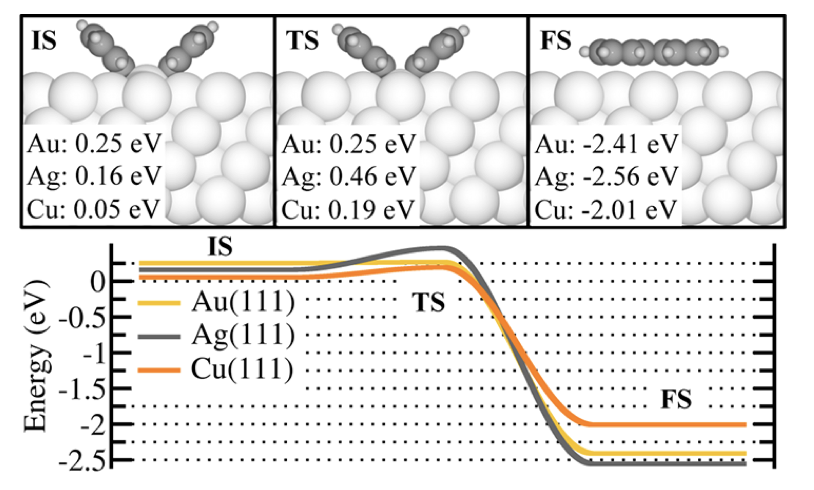
\includegraphics[width=0.85\columnwidth]{Fig/couplingenergy.png}
\caption{Coupling of two phenyls on Au(111), Ag(111), and Cu(111). The top panel depicts structures of the initial (IS), transition (TS) and final (FS) states on Ag(111). The energy of each state is shown relative to the most stable configuration of a single phenyl group on the respective metal surface. Adapted from Ref.~\cite{jacs2013}}
\label{fig:coupling}
\end{figure}

{\color{blue}

The investigation of this step has also been extended to a large scope of precursor choices, the monomer displays a equally decisive effect on the reaction condition of Ullmann coupling compared to the dehalogenation. STM technique offers a efficient approach to obtain the temperature information step. 
For example, 4-bromobiphenyl was proven to dimerize on Ag(111) surface at \SI{400}{\kelvin}, on Cu(111) at \SI{460}{\kelvin} and on Cu(110) at \SI{470}{\kelvin}~\cite{ullmann_92}.
1,3,6,8-Tetrabromopyrene has been reported to form C--C bond at \SI{473}{\kelvin} on Cu(111), at \SI{573}{\kelvin} on Au(111)~\cite{ullmann_93}.
While for molecule Cl--(ph)$_3$--Cl, it was found that this new bond is constructed at \SI{430}{\kelvin} on Cu(111), at \SI{470}{\kelvin} on Ag(111) and \SI{570}{\kelvin} on Au(111)~\cite{ullmann_93}.  
Summarizing the reaction condition of various monomers other than halobenzene  dimerizing on copper, silver and gold surface, we can conclude that the energy barrier for formation of C--C bond should decrease by the order Au $>$ Cu $>$ Ag. 

}

\iffalse
STM images, DFT calculation 2,5-diiodo-3,4-ethylenedioxythiophene Cu(110) dehalogenation RT, 200 degree polymerizaiton
Step-by-step growth of epitaxially aligned polythiophene by surface-confined reaction

STM image fast-XPS 1,4-dibromobenzene dehalogenation RT, 230 degree polymerization.
An unexpected organometallic intermediate in surface-confined Ullmann coupling

tribromoterthienobenzene
Au(111) 100 degree debromiantion, 200 degree most debromination finish, 400 degree C--C
Ag(111) RT debromination and C--Ag--C bridge network. 300 degree C--C formation
Cu(111) RT debromianton and C--Cu--C, 200 degree C--C
Surface-mediated assembly, polymerization and degradation of thiophene-based monomers

dibromo-p-terphenyl
STM image with step increasing temperature RT dehalogenation, form C--Cu--C
393 K C--C bond formation
Single-Molecule Resolution of an Organometallic Intermediate in a Surface-Supported Ullmann Coupling Reaction

1,3,6,8-Tetrabromopyrene
STM, XPS RT dehalogenation and C--Cu--C Cu(111)  473K C--C formation
473 K debromination and C--Au--C Au(111) 573K C--C formation
Comparing Ullmann Coupling on Noble Metal Surfaces:On-Surface Polymerization of 1,3,6,8-Tetrabromopyreneon Cu(111)and Au(111)

4-bromobiphenyl
STM Ag(111)
RT debrominattion and C--Ag--C.  400 K C--C
RT 460K Cu(111) 470 Cu(110) C--C
Steering Surface Reaction Dynamics with a Self-Assembly Strategy:
Ullmann Coupling on Metal Surfaces

Cl--(ph)$_3$--Cl
Cu(111) 80 degree C--Cu--C 160 degree coupling
Ag(111) 120 degree C--Ag--C 200 degree coupling
Au(111) 300 degree direct coupling
Ullmann Reaction of Aryl Chlorides on Various Surfaces and the Application in Stepwise Growth of 2D Covalent Organic Frameworks

Br−(Ph)3−Br confirm C--Au--C is not stable
Molecules−Oligomers−Nanowires−Graphene Nanoribbons: A Bottom-Up Stepwise On-Surface Covalent Synthesis Preserving Long-Range Order

1,3,5-tris(4-bromophenyl)benzene
temperature-programmed X-ray photoelectron spectroscopy (TP-XPS) + STM
250-290K debromination 300-420 C--C Ag(111)
500-600K C--C, no C--Au--C form
The Role of Kinetics versus Thermodynamics in Surface-Assisted Ullmann Coupling on Gold and Silver Surfaces
\fi



{\color{blue}
If the monomers contain more than one functional group, the Ulmann coupling proceeds further with the formation of trimers~\cite{jacs2016}, oligomers~\cite{ullmann_53, ullmann_56} or polymers~\cite{ullmann_43, ullmann_54, ullmann_55}. DFT modeling of the dimerization and trimerization of 1,4-dibromobenzene on Cu(100) surface shows that the activation energy for the C--C bond formation is \SI{0.89}{\electronvolt} and \SI{0.55}{\electronvolt}, respectively~\cite{jacs2016}. The consequent C--C formation leads to covalently bonded conjugated structure, which has also been validated with STM and fast-XPS in experiment. At \SI{470}{\kelvin}, alternating lines of poly(para-phenylene) will be comstructed from 1,4-dibromobenzene will through Ullmann coupling on Cu(110)~\cite{acsnano2013}. A growing number of multihalogen precursors are reported capable of forming 1D or 2D covalently conjugated structure on surface by further increasing the temperature after the C--C formation, such as polythiophene from 2,5-diiodo-3,4-ethylenedioxythiophene on Cu(110) at above \SI{470}{\kelvin}~\cite{ullmann_95}, more details have been discussed in our previous paper~\cite{ullmann_44}.
}


%\begin{figure*}[ht]
%\centering
%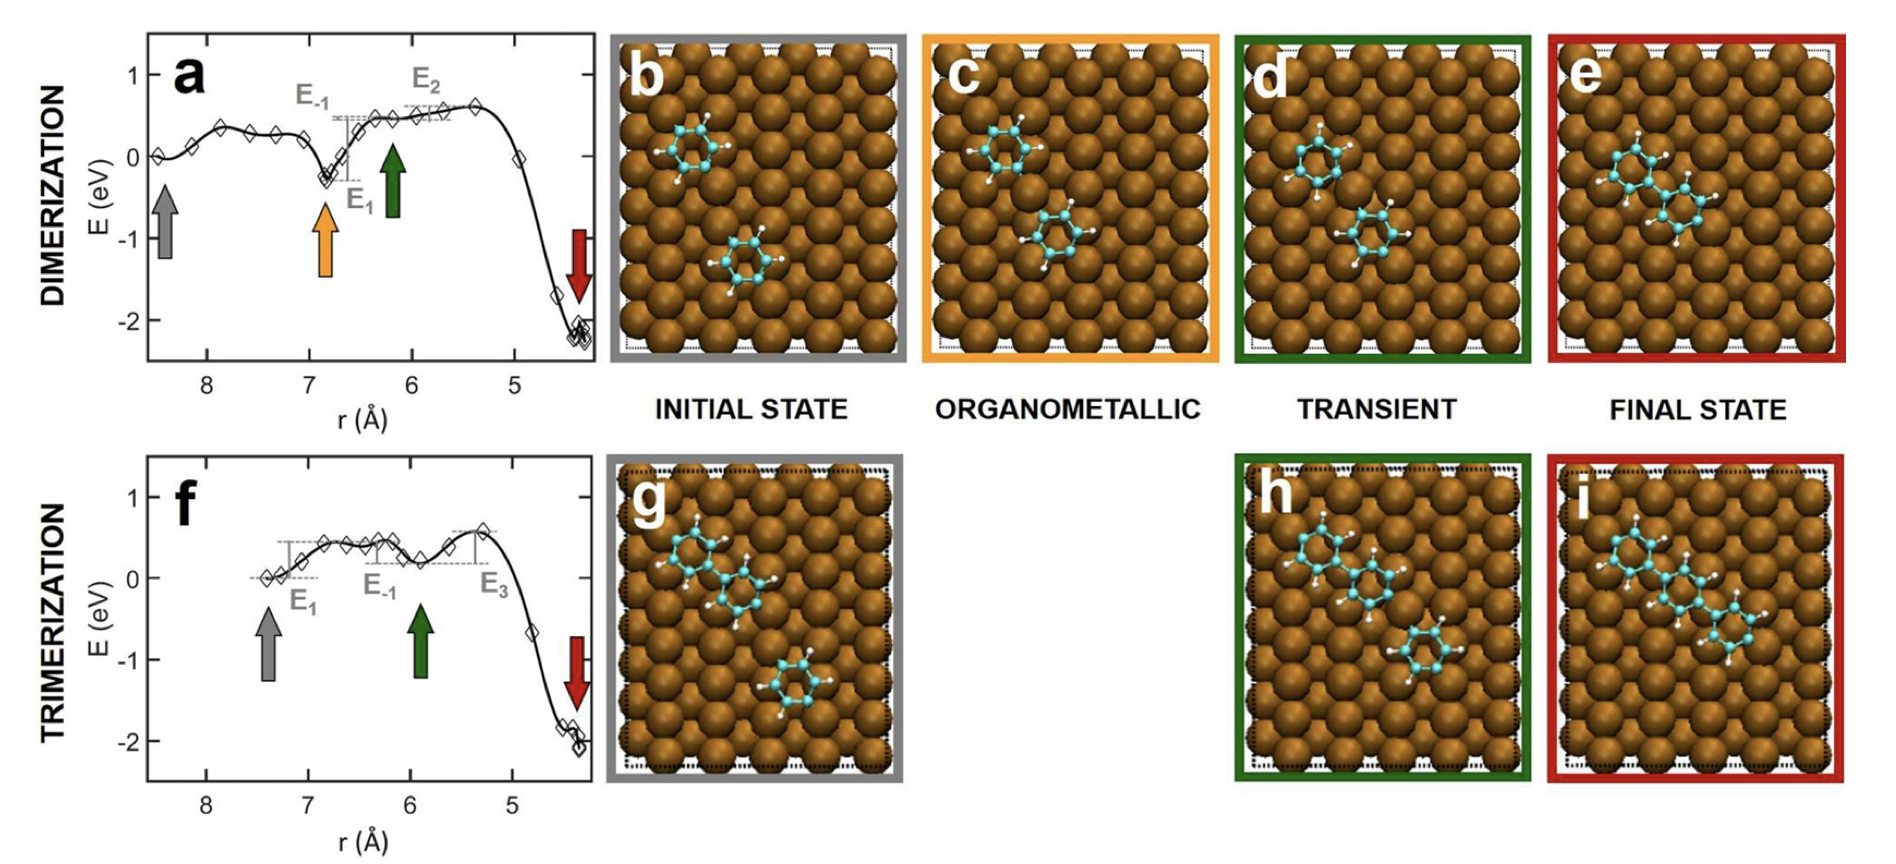
\includegraphics[width=1.0\textwidth]{Fig/Dimer_trimer.png}
%R1111: What metal is this. Better captions are required for all figures. Chemical identity of all species must be clear from the figure.
%\caption{Coupling barriers between (a) two monomers (dimerization) and (f) a monomer and a dimer (trimerization), respectively. The length (r) indicated in angstrom is the distance between the centers of the aromatic rings which undergo covalent coupling. The geometries of the most significant states (initial, organometallic intermediate, transient, and final) are reported in panels b--e and panels g--i for the dimerization and trimerization, respectively. The colors of the frames correspond to the arrows in panels a and f.}
%\label{fig:dimer}
%\end{figure*}
%

%ZZ0223 deleted: The general trend [RZK0122: is it really true for all metals?] is that the final C--C bond formation step requires the highest temperature among all other steps of the coupling process~\cite{Naturenano2007, ullmann_70, ullmann_71}. For example, for dichlorobenzene, dibromobenzene and diiodobenzene on Cu(110), the formation of C--C bond requires a temperature ranging from \SIrange{410}{450}{\kelvin}, which is noticeably higher than the \SIrange{170}{370}{\kelvin} temperature needed for the dehalogenation~\cite{ullmann_44}. 
RZK0122: The following sentence is inconsistent with the previous section.
On other type of Cu surface, as well on Ag and on Au surface, a higher annealing temperature for C--C coupling has also been
reported than dehalogenation steps~\cite{Naturenano2007, ullmann_70, ullmann_71}.

{\color{blue}

RZK0122: The following sentence is also inconsistent with the previous section. It should be explained and placed in the next section, where all steps analyzed together.  
Comparative analysis of different metal surfaces shows that the C--C bond formation requires \SIrange{330}{420}{\kelvin} temperature on Ag surface and \SIrange{500}{600}{\kelvin} on Au surface~\cite{ullmann_51}. On Cu, the temperature range is usually lower than on Au but higher than on Ag. This indicates that the energy barrier of the formation of C--C bond step on the three metal surfaces should follow Au $>$ Cu $>$ Ag. }


%RZK0426: The same analysis from the bond strength perspective could be useful. Ignore this comment for now.

\subsubsection{Summary on mechanism of surface Ullmann Coupling}

\begin{table*}
\centering
\begin{tabular}{ |p{5.3cm}|p{2cm}|p{2cm}|p{2cm}|p{2cm}|p{2cm}|p{2cm}|  }
 \hline
 \multicolumn{7}{|c|}{Temperature for steps in Ullmann coupling (\si{\kelvin}) } \\
 \hline
 \multicolumn{1}{|c|}{Step} & \multicolumn{3}{|c|}{Dehalogenation + C--M--C} & \multicolumn{3}{|c|}{C--C formation} \\
 \hline
 \diagbox[width=5cm]{Precursor}{Metal}  & Cu &Ag & Au & Cu &Ag & Au\\
 \hline
 Iodobenzene               &175\cite{sur_sci01} &200\cite{sur_sci02} &200-250\cite{sur_sci03} &350\cite{ullmann_68} &300-370\cite{ullmann_68} &250\cite{sur_sci03}\\
 Bromobenzene\cite{ullmann_67}  &160 &$\leq$ 197\cite{sur_sci02}  &  &350  &$\leq$ 350\cite{sur_sci02}  & \\
 dichlorobenzene &420\cite{ullmann_52} & & &470\cite{ullmann_52} & & \\
 dibromobenzene  &$\leq$ 300\cite{ullmann_52} & & &470\cite{ullmann_98}  & & \\
 diiodobenzene   &$\leq$ 300\cite{ullmann_52} & & &500 \cite{ullmann_88} & & \\
 1,4-dihexyl-2,5-diiodobenzene\cite{chemeurope2017} &$\leq$ 300 &$\leq$ 300 &No &390 &$\leq$ 300 &401\\
 Tribromoterthienobenzene\cite{ullmann_97}  &$\leq$ 300 &$\leq$ 300 &370-470 &470     &570 &670\\
 1,3,6,8-Tetrabromopyrene\cite{ullmann_93}  &$\leq$ 300 &    &473     &473     &    &573\\
 4-bromobiphenyl\cite{ullmann_92}           &$\leq$ 300 &$\leq$ 300 &        &460-470 &400 &   \\
 Cl--(ph)$_3$--Cl\cite{ullmann_93}          &350 &390 &No      &430     &470 &570\\
 1,3,5-tris(4-bromophenyl)benzene\cite{ullmann_51}  &  &250-290 &No & &300-420 &500-600\\
 \hline
\end{tabular}
\caption{Summary reaction conditions of multiple precursors on surface Ullmann coupling. RZK0426: Are these all (111) metal surfaces? Why some references are included in the first column?}
\label{table:exp-temp}
\end{table*}

{\lock

The effect of halogens and metals on each step of the surface Ullmann coupling reaction mechanism has been investigated both experimentally and computationally. The experiment condition of Ullmann coupling of multiple precursors on copper, silver and gold surface are listed Table~\ref{fig:temp}.

%\begin{figure}[ht]
%\centering
%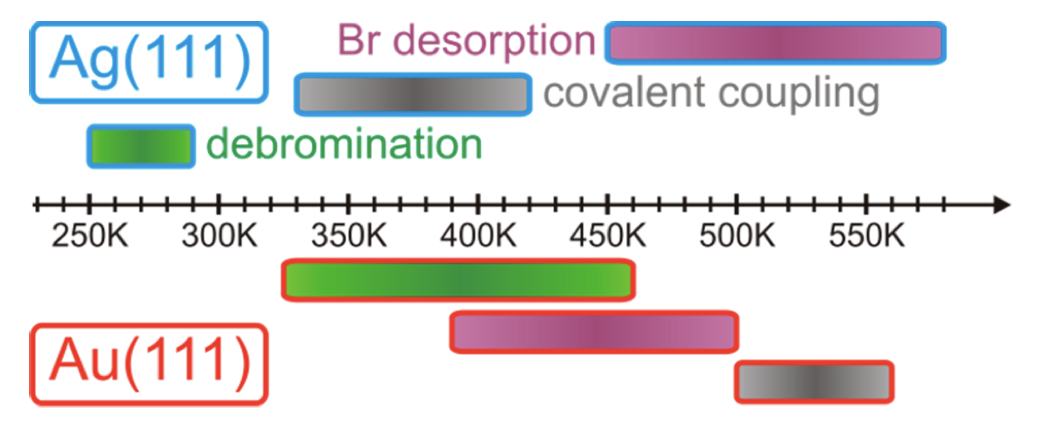
\includegraphics[width=0.75\columnwidth]{Fig/steptemp.png}
%\caption{Overview and Comparison of the Temperature Ranges for Debromination (Green), Covalent Coupling (Gray), and Thermal Desorption of Bromine (Violet) on Ag(111) (Top) versus Au(111) (Bottom) As Deduced from Both Br 3d and C 1s TP-XPS Data. Adapted from Ref.~\cite{ullmann_51}. RZK0426: Discuss creating our own figure summarizing temperatures and theoretical calculations for monosubstituted benzenes: 3 halogens and 3 metals. In its present form, the figure is not suitable for the introduction.}
%\label{fig:temp}
%\end{figure}

The onset temperatures of the dehalogenation and C--C bond formation steps are ultimately determined by the surface reactivity. Since carbon-metal steps are formed during the first step and broken during the second step the energy barriers for these two steps are often anticorrelated~\cite{jacs2016}. 
%
{\comm RZK0426: Dima's comment on the previous sentence: ``I don't see logic of such deduction.'' Dima's clarification is necessary because the idea for this sentence is taken directly from~\cite{jacs2016}. Perhaps the wording of the previous sentence needs to be improved? Examples are given below.}
%
On surfaces such as Au(111), where the dehalogenation barrier is high, the barrier for ejecting the metal atom from the organometallic bridge structure is often so low that the bridge state is rarely detected. In contrast, on surfaces such as Cu(110) and Cu(111) where the dehalogenation barrier is low, high temperature is required to convert the intermediate states into dimers, oligomers or polymers.
%
{\comm RZK0426: Dima's comment: ``It's not so much because C-C formation requires higher T on Cu than Au (not sure that's the case), but that C-X cleavage happens below RT on Cu, thus depositing at RT gives you directly the intermediate.'' A clarification is necessary.}

%RZK0426: It was decided to summarize halogen desorption here.
The high binding energy of halogen atoms on the surface -- calculated to be \SI{2.8}{\electronvolt} on Au(111) and \SI{3.1}{\electronvolt} on Cu(111)~\cite{RZK0426-reference-halogen} -- indicates that they are hard to desorb and remain on metal surfaces as by products of the reaction. It has been shown that such halogen atoms hinder the diffusion, coupling and polymerization of aryl species~\cite{ullmann_64,ullmann_65}. Therefore, removing halogens and other byproducts of on-surface Ullmann coupling is of great significance for creating well-ordered polymers for electronic devices.

}

{\comm RZK0426: Are there any other general trends that can be described here?}

\subsection{Role of adatoms in the surface Ullmann coupling} 

{\lock

Metal surfaces are not perfect, well-ordered structures. Even single-crystal metal surfaces are not free of defects ranging from three-dimensional defect such as pores~\cite{ullmann_72} and cracks~\cite{ullmann_73} to planar defects such as twin boundaries~\cite{ullmann_74} and stacking faults~\cite{ullmann_75}, line defects such as dislocations~\cite{Ullmann_76} and to point defects such as adatoms~\cite{Ullmann_77} and vacancies~\cite{ullmann_78}.
%RZK0507: restore the figure after the sentence if Dima insists (Fig.~\ref{cyrstal_surface}).

In the process of Ullmann coupling, reactants, intermediates and final products interact directly with metal atoms on the surface and, therefore, can be affected by surface defects. 
In fact, there is a growing body of evidence that adatoms can even be created during the reaction. 
Quantifying the extent to which adatoms and other imperfections of the metal surface influence the thermodynamics and kinetics of the Ullmann coupling can suggest new strategies for surface optimization, leading, in turn, to better defect-free assembly of two-dimensional polymers. 

%RZK0426: This figure appears in wikipedia. It is relatively simple and represents ``general knowledge''. I suggest removing it from the first article and perhaps also from the review.
%\begin{figure}[htb]
%\centering
%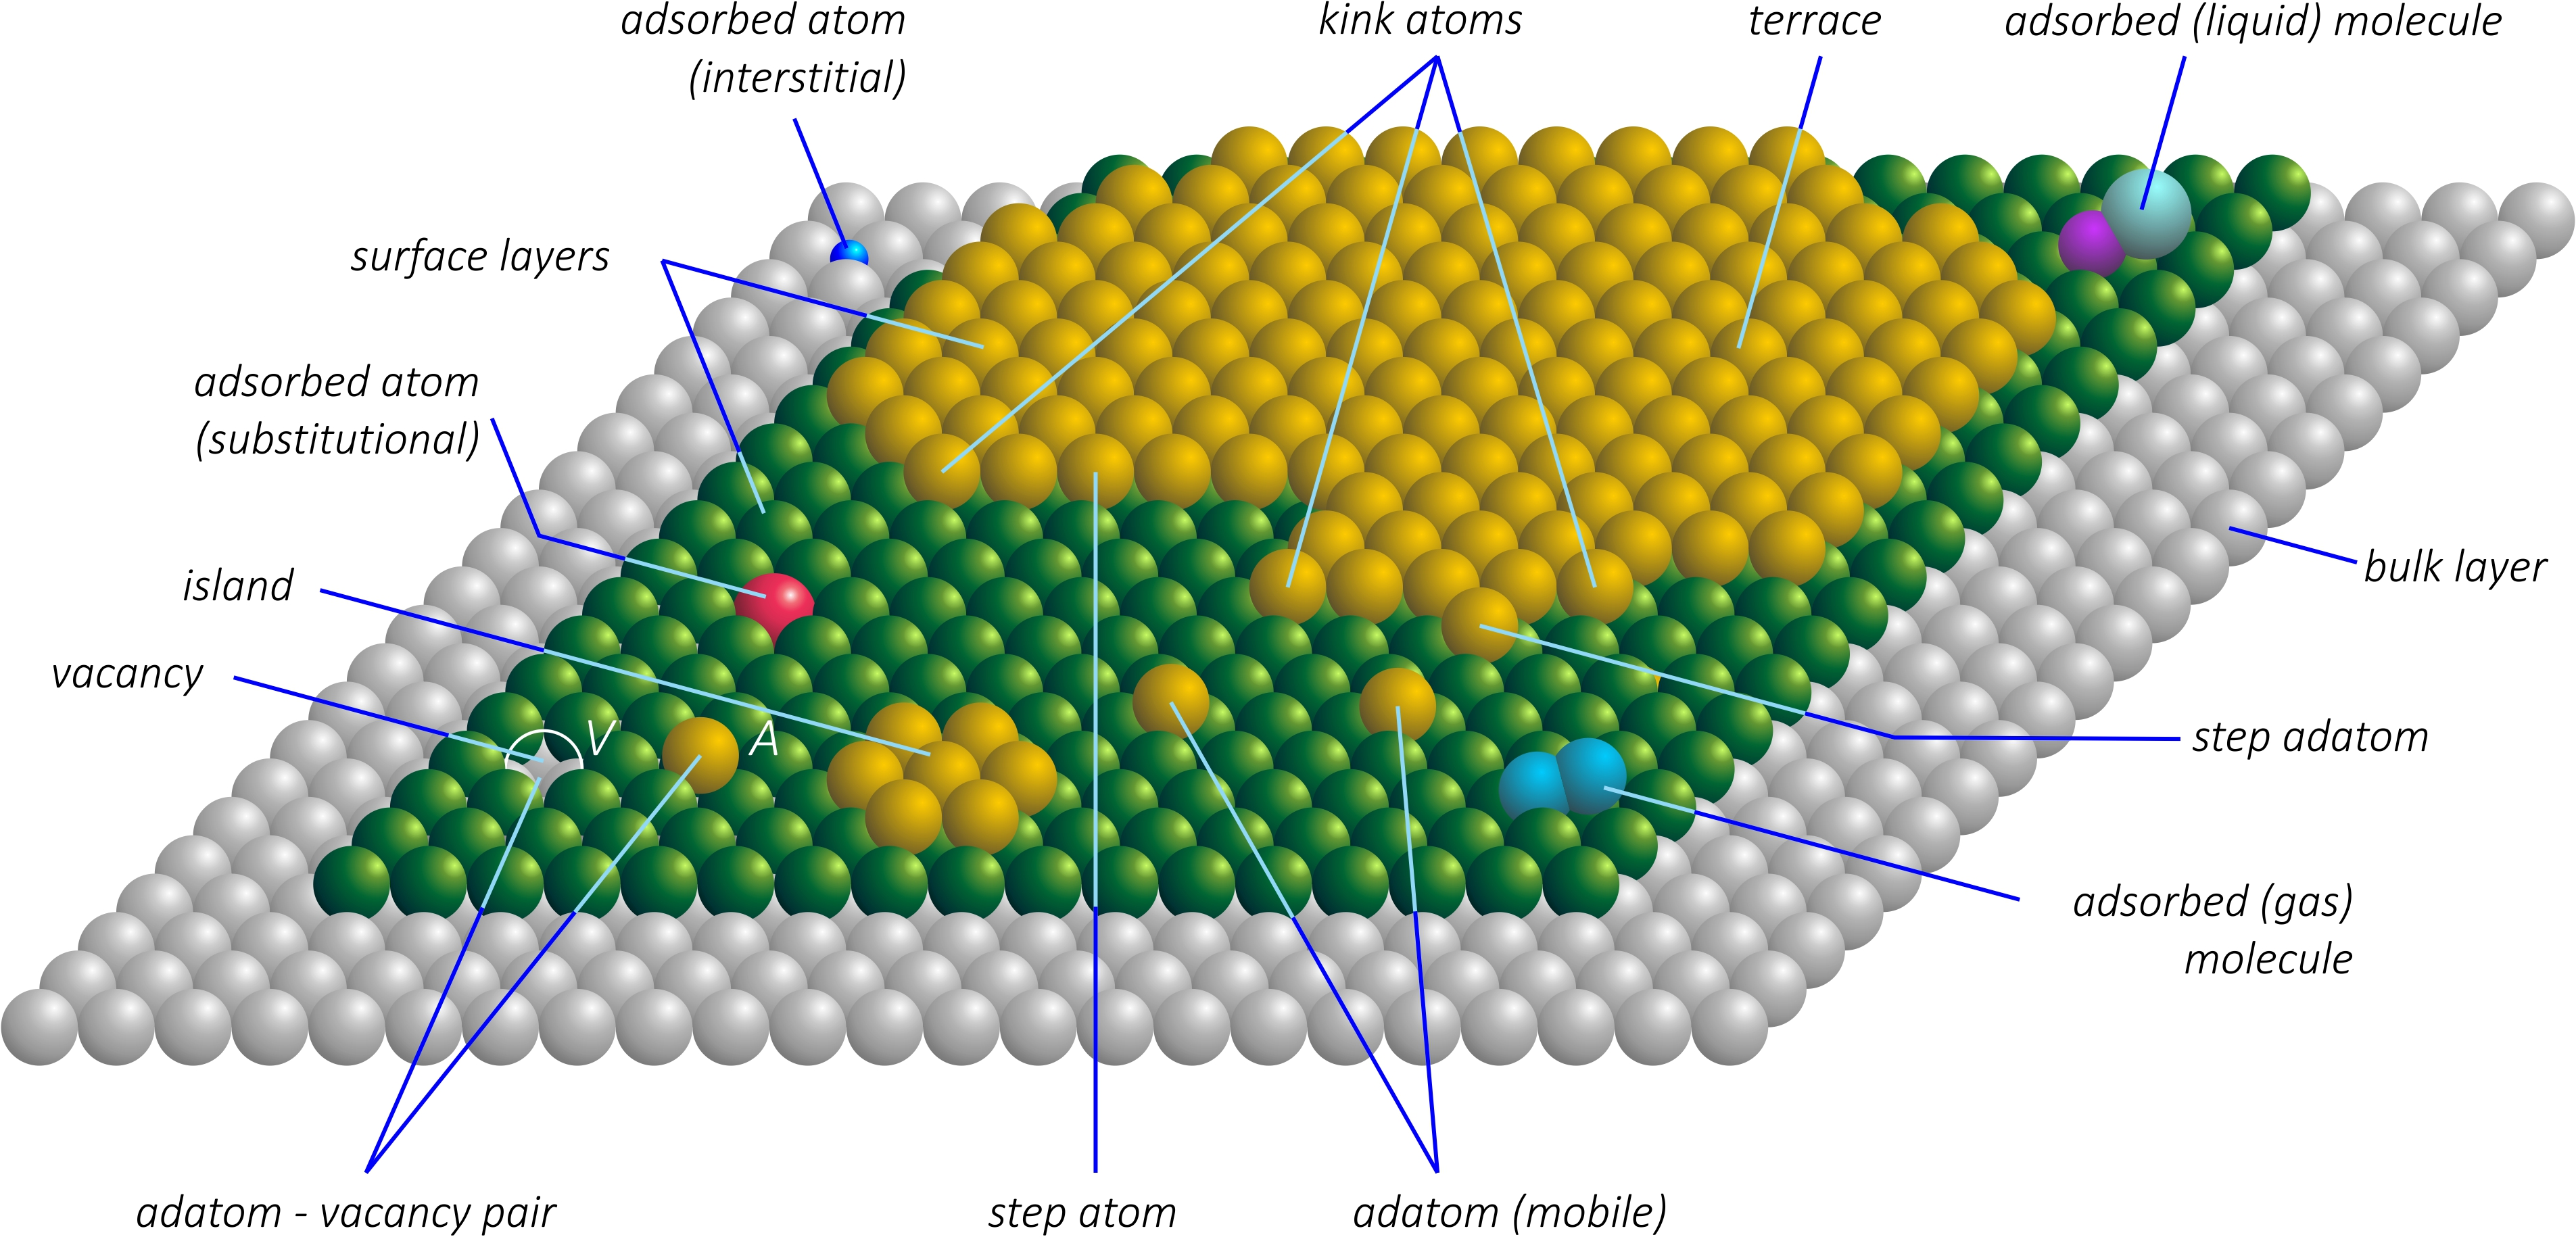
\includegraphics[width=0.4\textwidth]{Fig/Crystal_surface.jpg}
%\caption{A model of crystal surface. Adapted from Ref.~\onlinecite{ullmann_49}.}
%%RZK1221: Ignore at the moment. Remove the figure or find/create better figure. The text is almost invisible in this figure. 
%\label{cyrstal_surface}
%\end{figure}

%Surface metal atoms that affect and participate in the Ullmann coupling have different \emph{nature} and \emph{origins}.
%Atom's nature describes its immediate environment. 
To formalize discussion of the nature of surface atoms, metal atoms located within the first layer of atoms of the ideal surface will be referred to as \emph{ideal-surface} atoms. In contrast, \emph{adatoms}, according to the commonly accepted definition, lie on top of the layer of ideal-surface atoms. In this work, adatoms are differentiated according to their origin into \emph{pre-existing} and \emph{extracted} adatoms. %The origin of pre-existing atoms is irrelevant, not specified, or not known. 
Extracted adatoms are known to have been lifted from their lattice sites and placed on top of the surface leaving a surface vacancy behind~\cite{ullmann_96}. Here, \emph{vacancy} refers exclusively to vacant lattice positions on the surface, not in the bulk.

%The nature of metal atoms and the origin of adatoms have been explored experimentally and computationally.
%For origin(1), it has been reported that the onset of the vacancy-adatom formation take place on Cu(111) surface was around 900 K by molecular dynamics~\cite{ullmann_50} , which is much higher than the temperature required by surface Ullmann coupling reaction, as shown in Fig.~\ref{fig:2Dgasn}~\cite{ullmann_50}. This could be the evidence that there would not be new adatoms formation due to the thermal fluctuations as the surface Ullmann coupling proceeds. 

It is well known that Cu adatoms are created on clean Cu(111) surface by thermal fluctuations~\cite{ullmann_79, ullmann_58}. Silver and gold adatoms can be also be created especially near {\comm line, planar?} defects such as {\comm step edges, kinks?}~\cite{ullmann_84, ullmann_85}. 
It has been calculated~\cite{chemeurope2017} that the formation of an adatom on clean Cu(111), Ag(111) and Au(111) surfaces requires substantial energy of \SI{1.71}{\electronvolt}, \SI{1.12}{\electronvolt} and \SI{1.15}{\electronvolt}, respectively, making the equilibrium concentration of adatoms on clean surfaces negligibly small.  
%{\comm RZK0426: Dima's comment: ``What is known about concentration of ad-atoms on various single-crystal surfaces at RT?'' RZK agrees that stating this number is desirable. ZZ: ``I did not find it with a long time, will finish it later.''}%
Pre-exisiting adatoms have previously been observed to participate in metal organic coordination networks~\cite{ullmann_80, ullmann_81, ullmann_82, ullmann_83}, which suggests that they can play an important role in on-surface Ullmann coupling.

%\begin{figure}[ht]
%\centering
%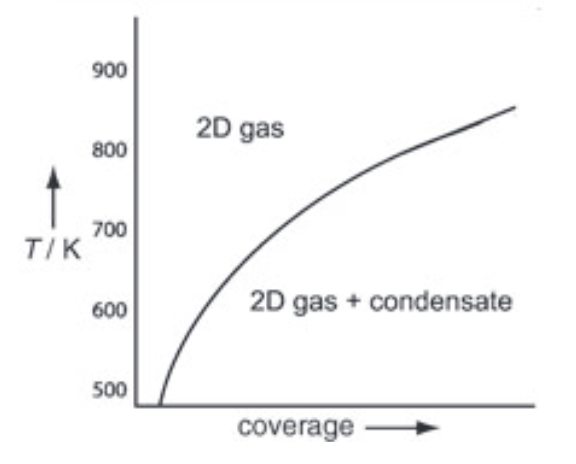
\includegraphics[width=0.75\columnwidth]{Fig/2D-gas.png}
%\caption{Schematic diagram of 2D adatom gas phase and condensed phase (islands) %coexisting at elevated temperatures for metal-on-metal systems.}
%\label{fig:2Dgas}
%\end{figure}

}

\subsubsection{Dehalogenation}

\begin{figure}[htb]
\centering
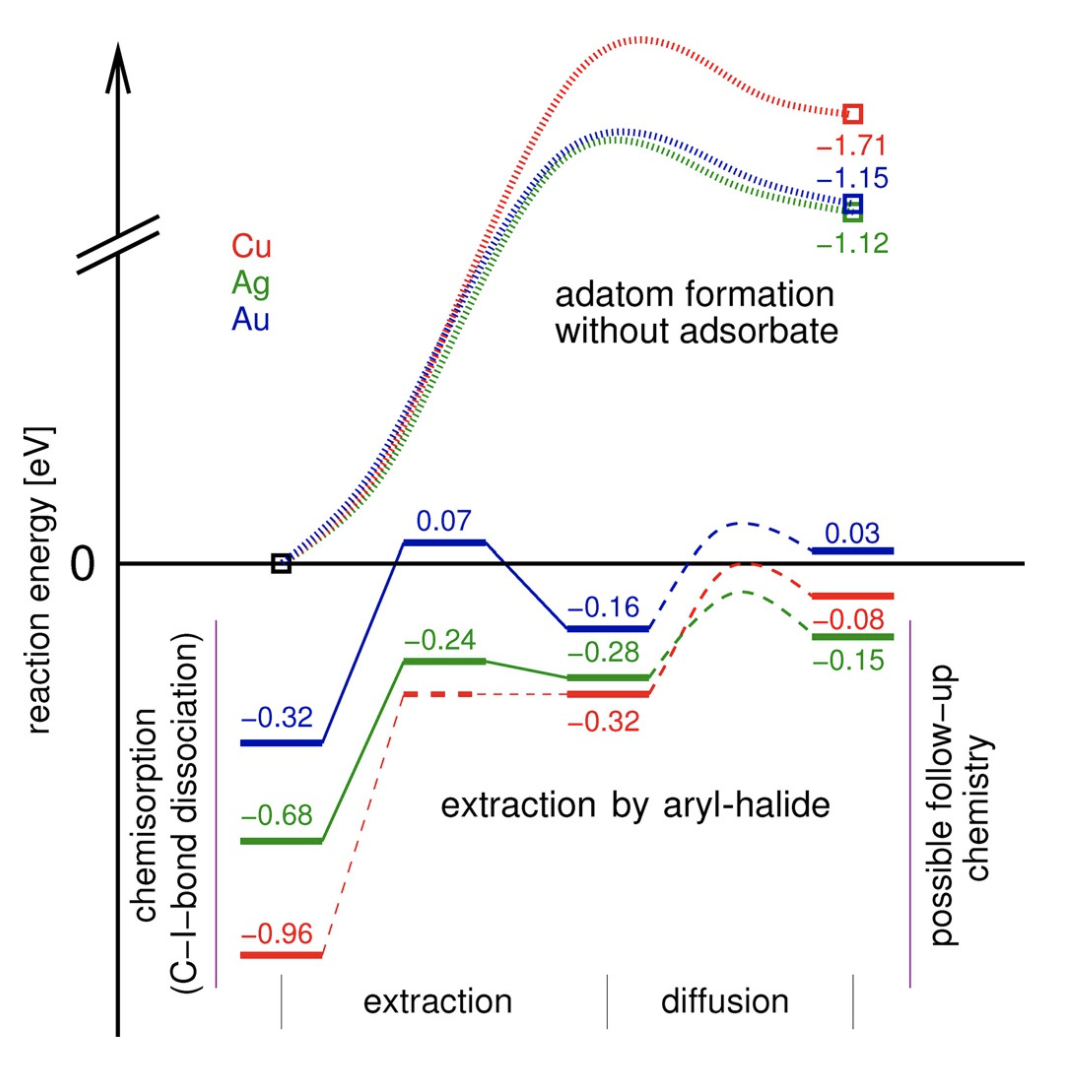
\includegraphics[width=0.75\columnwidth]{Fig/Adatom-formation.png}
\caption{Graphical comparison of the energetics of the adatom formation without adsorbate (top half) to the extraction by aryl–halide process (lower half).Values for Cu are shown in red, for Ag in green and for Au in blue. The extraction-by-arylhalide process starts from the dissociated iodobenzene. Dotted lines indicate parts of the energy profile that have not been quantitatively resolved. Adapted from Ref.~\cite{chemeurope2017}}
\label{fig:3}
\end{figure}

{\lock

It has been suggested based on results of STM investigation and DFT calculations that adatoms can be created after the dehalogenation of aryl precursors in the initial stages of the on-surface Ullmann reaction. As shown in Fig.~\ref{fig:3}, the calculated energy required to lift an ideal-surface atom and place it on the surface is reduced to \SI{0.64}{\electronvolt}, \SI{0.40}{\electronvolt} and \SI{0.16}{\electronvolt} for Cu(111), Ag(111) and Au(111) surfaces, respectively, if the extracted adatom is bonded to iodine and phenyl fragments -- the products of the dehalogenation of a iodobenzene molecule~\cite{chemeurope2017}. {\comm RZK0506: The energy for Cu appears to be wrong. Read the article and discuss the energies with me.}
%
It has also been concluded that the significantly reduced adatom extraction energy (compared to that on the clean surface) can be fully compensated by the release of comparable amount of energy in the preceding dehalogenation step, making the combined dehalogenation and extraction essentially thermo-neutral on these surfaces.

%RZZK: For future comparison in RnD: extraction here is still hugely endothermic, unlike the extraction at later steps.

%Dehalogenation of iodobenzene will result in phenyl-metal species, the energies of this interaction with full extraction of ideal-surface atom were calculated to be \SI{0.64}{\electronvolt}, \SI{0.40}{\electronvolt} and \SI{0.16}{\electronvolt} for Cu, Ag and Au surfaces, decreased by \SI{1.07}{\electronvolt}, \SI{0.72}{\electronvolt} and \SI{0.99}{\electronvolt}, respectively. 

%Till now it can be concluded that dehalogenation lowers the energy required for creation of adatoms from ideal-surface atoms on a metal surface. 
%The direct use of pre-existing adatoms should ideally cut down the energy barrier for this step compared to ideal-surface atoms.
%Dima: This makes no sense. The energy of a step X is not affected by existence of an alternative step Y. (ZZ: a pre-existing adatom will affect the initial geometry of dehalogenation.)
%However, few work has been related to pre-existing adatoms in dehalogenation.

}


\subsubsection{Diffusion}

\begin{figure}[hbt]
\centering
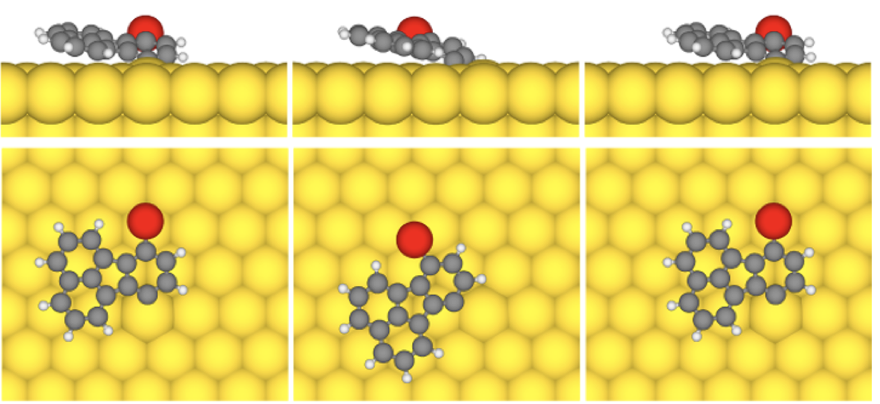
\includegraphics[width=0.75\columnwidth]{Fig/Diffusion_path.png}
\caption{Top and side view of the initial, transition and final geometries of bromofluoranthene molecule diffuse. Adapted from Ref.~\cite{jpcc2018}}
\label{fig:diff}
\end{figure}

%The diffusion process is involved in the interaction between single precursor group and metal atom. 
%In 2018, Nagoya \textit{et al.}~\cite{jpcc2018} investigated the mechanism of Ullmann coupling of 7,10-dibromofluoranthene (Br$_{2}$FL) on Au(111) via DFT calculations. Compared to simple phenyl rings that tend to form ~$36^\circ$ tilt angle with Cu(111) surface~\cite{pccp2010}, the monobromo FL with one Br atom removed would stay almost parallel to Au(111) surface due to steric repulsion between the large backbone of BrFL group and the substrate. And BrFL group was found to lift surface Au atom out by 1.9 \angstrom\ from its initial position, which is much larger than 0.16 \angstrom\ height lifted by a simpole phenyl ring, as shown in Fig.~\ref{fig:diff}.
%Ebeling \textit{et al.}~\cite{acsnano2019} also indicated 4-bromo-3$^{''}$-iodo-$p$-terphenyl group interacts with the Cu atom inside the surface, and would partially lift the Cu atom out from the surface while diffusing on Cu(111) surface. 
%
%Metal atoms of $nature(1)$ were proven to play a significant role in the diffusion of dehalogenated phenyl groups, the metal atoms that interact with phenly groups will be partially lifted from its original position, the lifting height is affected by the intensity of interaction between the phenyl group and metal atom. Formation of adatom of $origin(2)$ has not been reported in diffusion, which indicates that the interaction between phenyl group and metal atom in this step is not in the magnitude to fully extract a metal atom of $nature(1)$. 

{\color{blue}

There were no apparent proof that placing dehalogenated species on metal surface can form new adatoms from ideal-surface atoms. Most reports assumed that dehalogenated intermediates interact with ideal-surface atoms in diffusion process. The energy involved in this type of interaction is determined by the geometry of intermediates and type of metal atoms.

For single phenyl groups diffusing on Cu(111), ideal-surface copper atom is lifted only by \SI{0.16}{\angstrom} from its original position in diffusion~\cite{pccp2010}, the height is insufficient to create an adatom on surface by full extraction. With the molecular size increasing, the steric repulsion of precursor radical and surface can change the pattern of diffusing, the metal atom will be lifted higher and the precursor will stay more parallel to the surface. For example, DFT calculations revealed that bromofluoranthene radical (dehalogenated one bromide from dibromofluoranthene) will lift an ideal-surface gold atom up to \SI{0.5}{\angstrom} after dehalogenation~\cite{jpcc2018}. Then in the diffusion of this aryl radical on Au(111) surface, it will interact and adsorb different ideal-surface gold atom along the mobile path, the largest height each gold atom raised is up to \SI{1.9}{\angstrom} and the molecule remains almost parallel to Au(111) surface. Two bromofluoranthene radical diffusing to each other will adsorb a common gold atom and fully exact it out of first layer by \SI{2.2}{\angstrom} and leave a vacancy below, which suggests that the interaction between two these aryl radicals and gold atom is more intensive and enough to create an adatom compared to single aryl radical.

The evidence of pre-existing adatoms are involved in this step is not reported. It can be speculated that diffusion of aryl groups on metal surface can seldom create adatoms since the intensity of interaction between one dehalogenated species and metal atoms is not sufficient to fully extract ideal-surface atoms out.

}

\subsubsection{Formation of C--M--C structure intermediates} \label{sec:dimerized-adatom}

%The nature of the metal atoms in dimerized organometallic intermediate has been investigated through multiple approaches. Besides, it can be deduced that an metal atom of $nature(2)$, which is also an adatom of $origin(1)$ will exit above the first layer of surface before the surface Ullmann coupling reacion occurs. And this atom can attract two phenyl groups diffuse close to it and form the dimerized organometallic intermediate in this step. This type of formation might require less energy compared to the situation that two phenyl groups both interact with the same metal atom of $nature(1)$. The arguments on the nature and origin of metal atoms in this step are intense in the mechanism of surface Ullmann coupling.

%In 2017, Zint \textit{et al.}~\cite{acsnano2017} analyzed structures of intermediates in the polymerization of bromotriphenylene to bistriphenylene on Cu(111) surface using STM, AFM image and DFT calculations. Two computational models were compared: two triphenylene molecules bonded to an fully-out-of-surface adatom (a metal atom of $nature(2)$) and two precursors bonded to an atom partially lifted from Cu surface (a metal atom of $nature(1)$) as shown in Fig.~\ref{fig:5}. It has been concluded that the structures observed in AFM were more consistent with computational adatom ($nature(2)$) models. In particular, the C--C distance in organometallic intermediate was of 3.9 \angstrom\ measured by AFM, which was closer to the Cu adatom ($nature(2)$) model (3.86 \angstrom) compared to the partially-lifted Cu atom ($nature(1)$) model (3.42 \angstrom). Furthermore, the energy for formation of the adatom-containing intermediate from distant precursors was 1.74~eV lower than that of the intermediate with a partially lifted atoms. 

\begin{figure}[hbt]
\centering
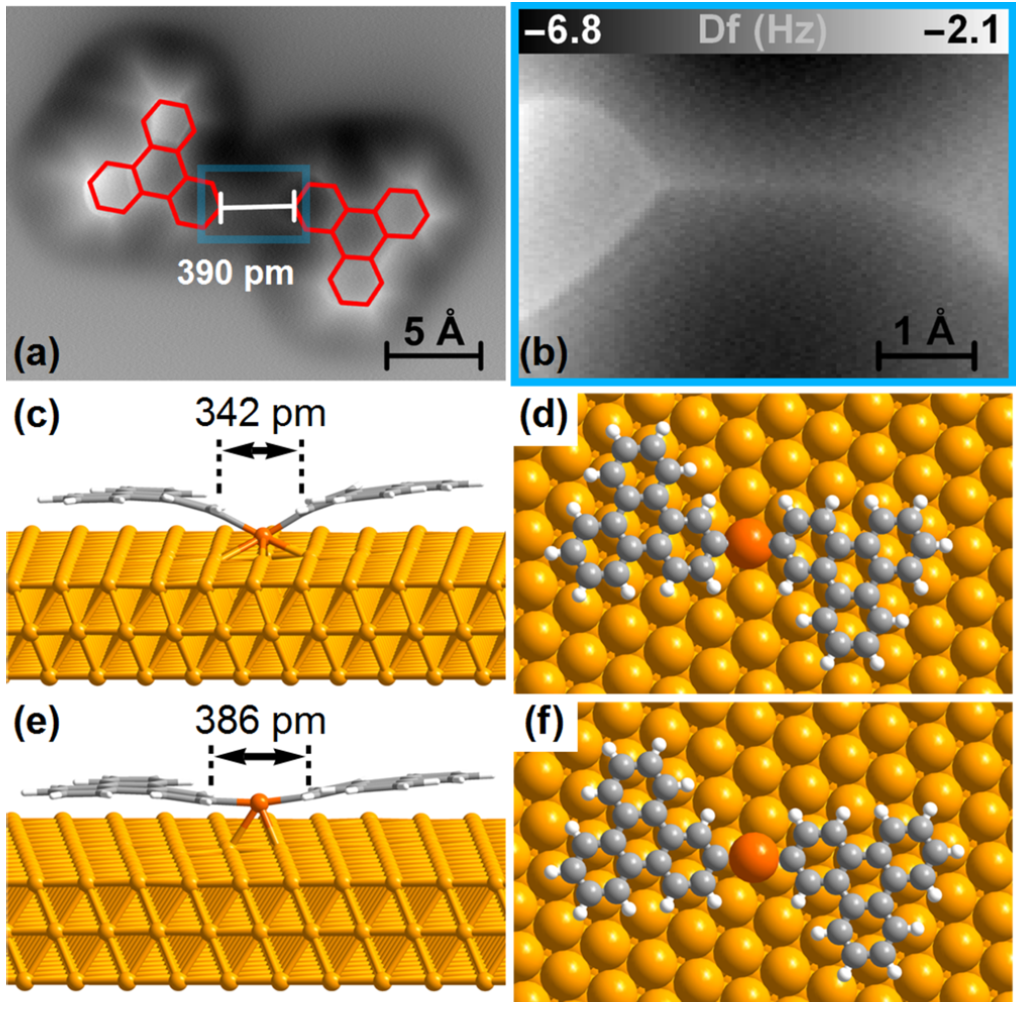
\includegraphics[width=0.75\columnwidth]{Fig/distance.png}
\caption{(a) AFM frequency shift image of intermediate with fit of structural model. (b) Zoom on intermediate bond ($cf$. blue box in a) imaged with decreased tip-sample distance ($\Delta$z = -70 pm with respect to image a). (c--f) DFT-D3 calculations [PBE-D3/ pw (PAW P)] for two different organometallic intermediate states (surface atom (c,d) vs adatom (e,f)). Adapted from Ref.~\cite{acsnano2017}}
\label{fig:5}
\end{figure}

%The origin the adatoms were later explored after the metal atoms in dimerized organometallic intermediates were proven to be of $nature(2)$, which is an adatom on surface. In 2019, the study of 4‐Bromo-3$^{''}$- iodo‐$p$‐terphenyl coupling on Cu(111), proved again that the Cu atoms in dimerized organometallic intermediates were adatoms (metal atoms of $nature(2)$) compared experiments with simulated AFM image[Fig.~\ref{fig:6}~\cite{acsnano2019}]. It was further suggested that these adatoms are generated by the extraction of two close single precursor groups (adatom of $origin(2)$), instead of pre-exsiting adatoms (adatoms of $origin(1)$) from a statistic study of all intermediates species in the surface Ullmann coupling.

\begin{figure}[ht]
\centering
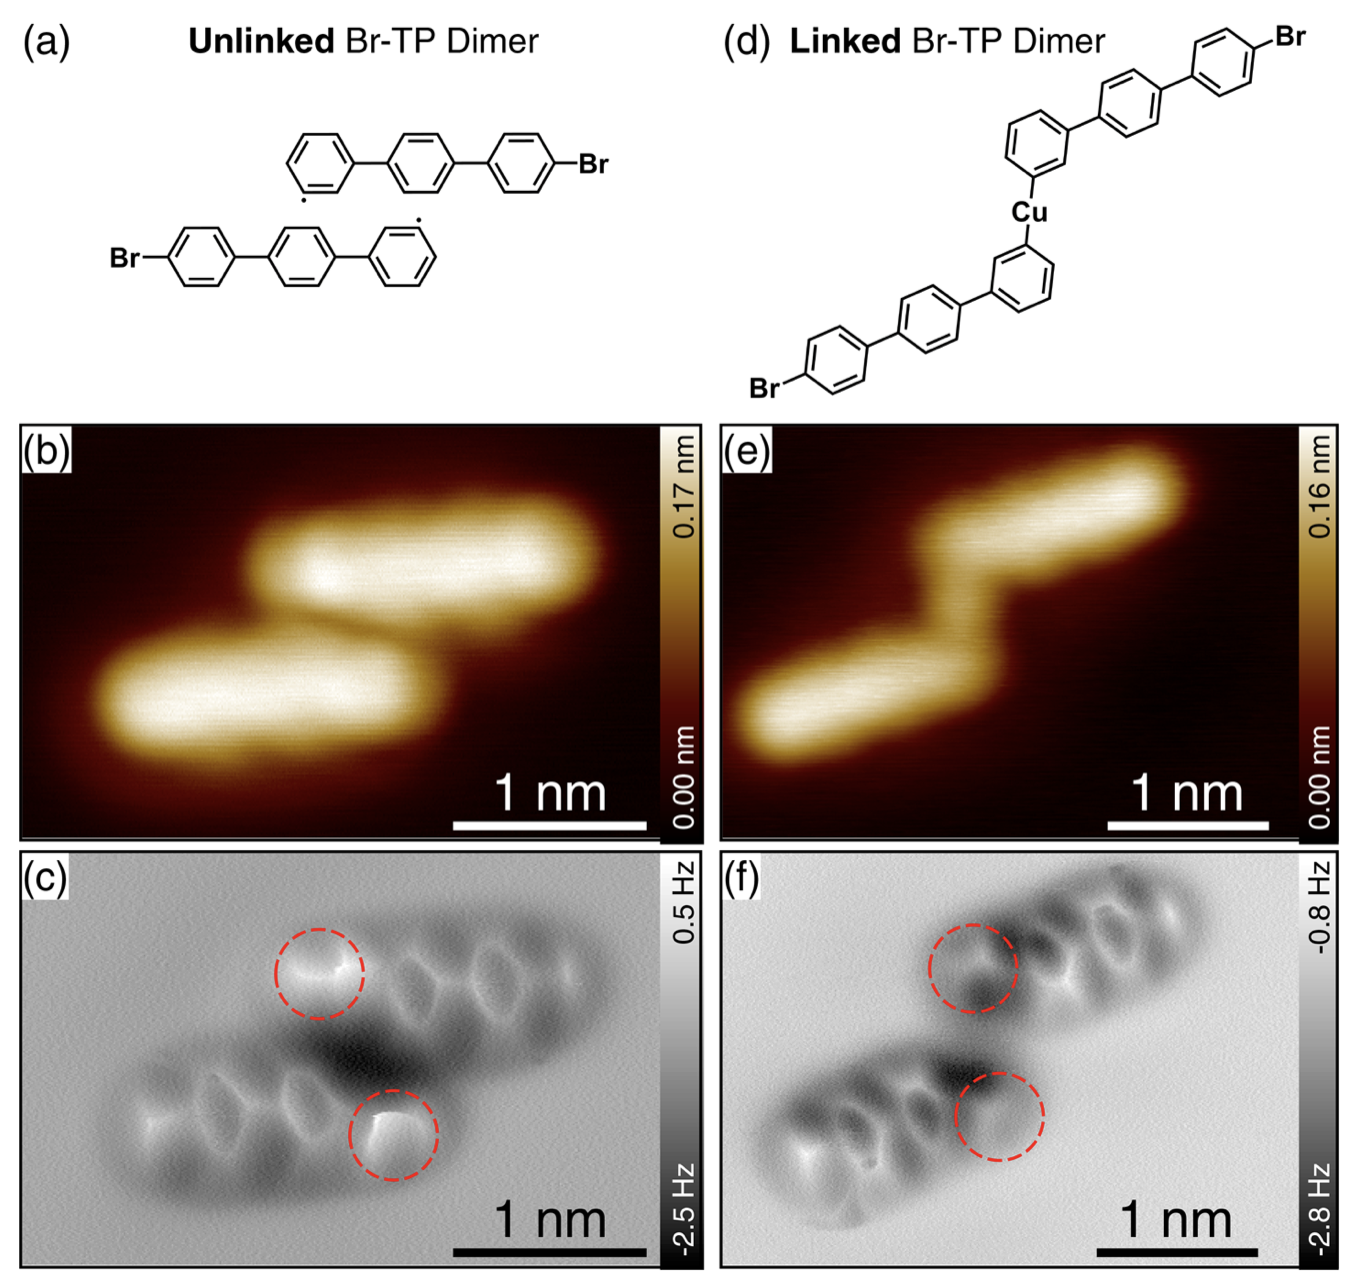
\includegraphics[width=0.75\columnwidth]{Fig/AFM_prove.png}
\caption{Molecular structures (top row), STM (middle row), and AFM images (bottom row) of 4‐Bromoterphenyl dimers on Cu(111). Two different types of dimers are observed, which are denoted as unlinked (left column) and linked dimers (right column). The STM image of the unlinked dimer reveals a dark region between the two molecules that separates them. Between the two molecules of the linked dimer a bright protrusion is observed in the STM scan that directly links them. The red dashed circles in (c) and (f) indicate the twisted phenyl rings, which lost their iodine atoms. Imaging parameters: (b) 200 mV, 30 pA, (e) 200 mV, 10 pA, tip height z = -100 pm (c) and z = -24 pm (f) with respect to a tunneling set point of 200 mV and 10 pA on Cu(111). Adapted from Ref.~\cite{acsnano2019}}
\label{fig:6}
\end{figure}

%The nature of metal atoms in dimerized organometallic intermediates has been proven to be an adatom. And further the origin of this adatom is of $origin(2)$, which indicates before the surface Ullmann coupling reaction occurs, the adatom is still a metal atom of $nature(1)$, stay in the first layer of metal surface. After it was selected from two phenyl groups in coupling procedure, it will be fully lifted out of the surface, become a new adatoms. The effect of metal atom in the last step --- formation of C--C bond was not investigated intensive compared to previous steps.

%%In addition, chlorinated prophyrin as precursor has also been deposited on Cu(111)~\cite{chematerial2019}. Based on DFT calculations, the Cu adatom mediated path is 3~eV lower than the direct dechlorination. And from STM image, some precursors are still intact at temperature of 400~K, which should be already dehalogenated at lower temperature. It proves that the Cu adatoms are the limiting agent [Fig.~\ref{fig:prophyrin}].

%\begin{figure}[ht]
%\centering
%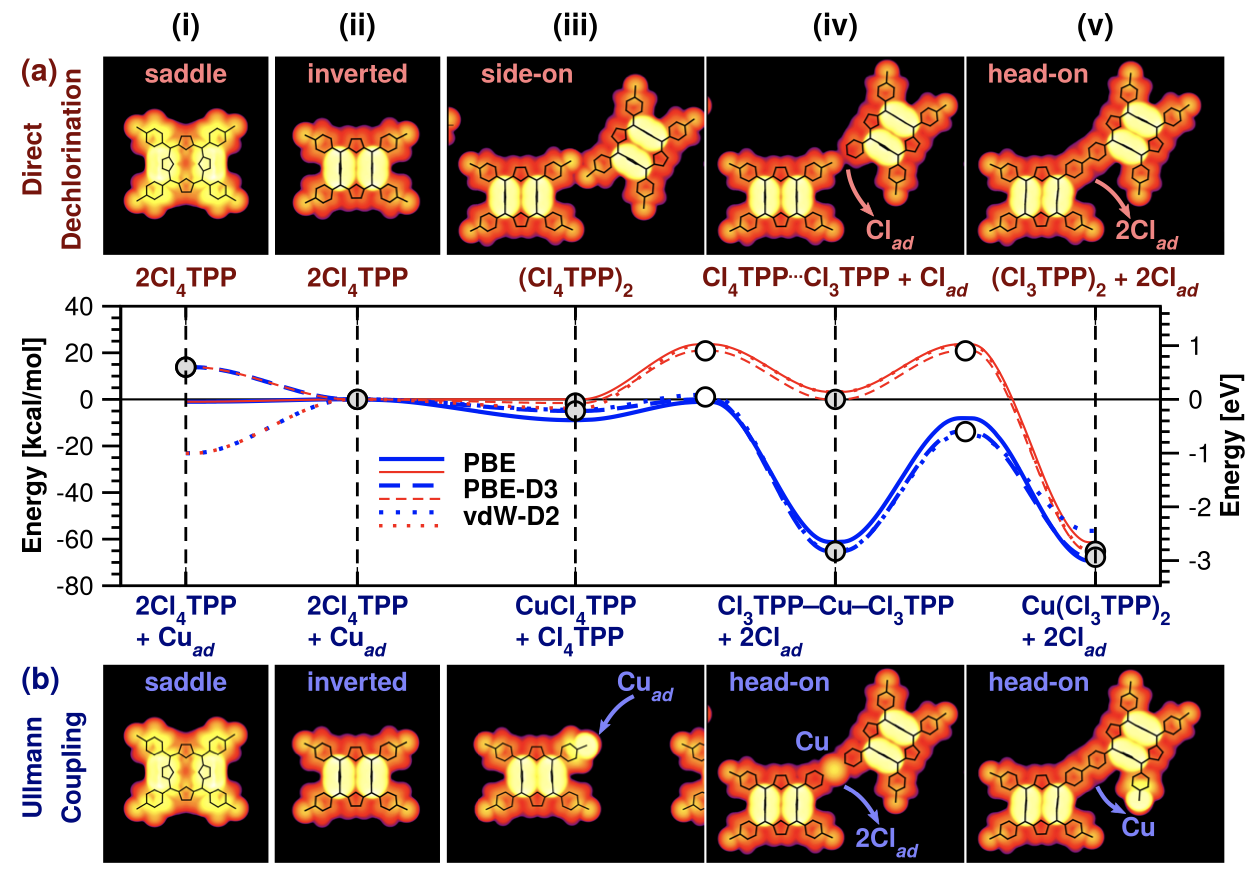
\includegraphics[width=0.4\textwidth]{Fig/Complete.png}
%\caption{STM simulations and DFT reaction profile for the (a) direct %dechlorination reaction (red lines) and (b) Cu adatom-mediated Ullmann coupling reaction (blue lines). For each process the energy are plotted of the (i, ii) precursors, (iii, iv) intermediates, (v) and final species (gray circles) and two transition states (white circles).}
%\label{fig:prophyrin}
%\end{figure}

%%ZHZH Dima suggests partial lifting should be discussed separately.
{\color{blue}
The mechanism of metal atoms participating in the formation of C--M--C bridges structure are intensively investigated. Multiple approaches have been used to figure out it is adatoms or ideal surface atoms that actually constitute the C--M--C bridge~\cite{acsnano2017}. 

\sout{It has been proven that two phenyl groups, after diffusing to adjacent position, will bind to the same ideal surface copper atom and form C--Cu--C structure on Cu(111)}~\cite{pccp2010, acsnano2019}.
\sout{Similar structure will be constructed on Ag(111) and Au(111) surface from phenyls and ideal surface silver and gold atoms.}

Fig.~\ref{fig:5} describes the C--Cu--C structure formed by two triphenylene moieties with a copper atom on Cu(111) surface using AFM and DFT methods~\cite{acsnano2017}. Two distinct simulation models are shown: (1) the copper atom in C--Cu--C structure comes from ideal surface atom as shown in (c) and (d). This ideal surface atom is partially lifted up from its original position in the first layer of metal; and (2) the copper atom in C--Cu--C is an adatom as pictured in (e) and (f). Two model are compared with AFM image on atomic properties. The distance between carbon and carbon in this C--Cu--C bridge in AFM, ideal surface model and adatom model are \SI{3.90}{\angstrom}, \SI{3.42}{\angstrom} and \SI{3.86}{\angstrom} respectively, which shows that the adatom model is more consistent with the molecule geometry in experiment. This is in agreement with DFT calculations showing that the energy for formation of C--Cu--C bridge structure from these precursors with adatom is estimated to be \SI{1.74}{\electronvolt} lower than with ideal surface atom, both from two chemisorbed dehalogenated radicals on Cu(111) surface as initial states. \sout{The metal atoms in C--M--C intermediate structure were proven to be adatoms with clear evidence for the first time. Then the pathway of emerging such adatoms was also reported.(Dima)} This proves that it is highly likely to be adatom that make up the C--M--C structure.

In Fig.~\ref{fig:6}, the STM and simulated AFM image of forming C--Cu--C intermediate structure from 4‐bromoterphenyl and copper atom are displayed~\cite{acsnano2019}. Based on the comparison of the experimental STM and simulated AFM image data, the metal atom participated in the C--Cu--C structure is again, proven to be adatoms rather than an partially lifted ideal surface atom. Furthermore, these adatoms, according to the statistic data, are created during the surface Ullmann coupling reaction by extracting the ideal surface atoms out instead of pre-existing adatoms before the coupling process.

In this step, the actual state of origin and nature of metal atoms involved still remains unclear. Previously works suggest that for some intermediates, there is compelling evidence to consider adatoms taking part in C--M--C intermediate structures. And the formation of such a bridge structure can serve as a feasible strategy to create adatoms on Cu(111) surface. However, as discussed in former section, the strength of interaction between aryl groups and metal atoms is defined both by the structure of aryl group as well as the type of metal atoms. Whether surface Ullmann coupling on different surfaces will proceed via the same adatom based mechanism still remains an open question.

}

%RZK0426: Has the statement below from jacs2013 been incorporated? 
%Furthermore, the presence of Cu adatoms may impact the self-assembly more than the poor diffusion on the atomically flat Cu(111) surface. These adatoms are known to have a great influence on selfassembly on Cu(111), where in many cases coordination bonds are formed instead of covalent networks.21 The Cu adatoms can also contribute to the covalent bonding of the nanostructure.22,23 (%ZZ maybe we should add this in the diffusion section in adatom part)

\subsubsection{Formation of the C--C bond}

{\color{blue}
For the last step, in which a C--C bond is constructed in the coupling. The role of metal atom in this formation has also been reported, but rarely compared to other steps discussed above. However, there are numerous unsolved questions in this step, such as the possibility of creating a brand new adatom from ideal surface adatom in this step, the final destiny of metal atom involved in reaction after Ullmann coupling is finished, the influence of adatom on further successive coupling.

The energy profile and geometry evolution of bromofluoranthene coupling to dimer has been investigated with CI-NEB calculations, as shown in Fig.~\ref{fig:7}. The height of common gold atom adsorbed by two aryl radicals is largest up to \SI{2.2}{\angstrom} in the C--Au--C bridge structure, which can be regarded as an adatom fully extracted and create a vacancy below. Then the height keep lowering with the reduce of distance between two unsaturated carbon atoms. In the end, the gold adatom return back to its original position along with the formation of dimer. It advises that the adatom created in C--M--C structure step will only exist until the completion of Ullmann coupling. It can not be conferred as a real creation of adatom, which can further diffuse on metal surface and be different from other ideal surface atoms.
}


\begin{figure}[ht]
\centering
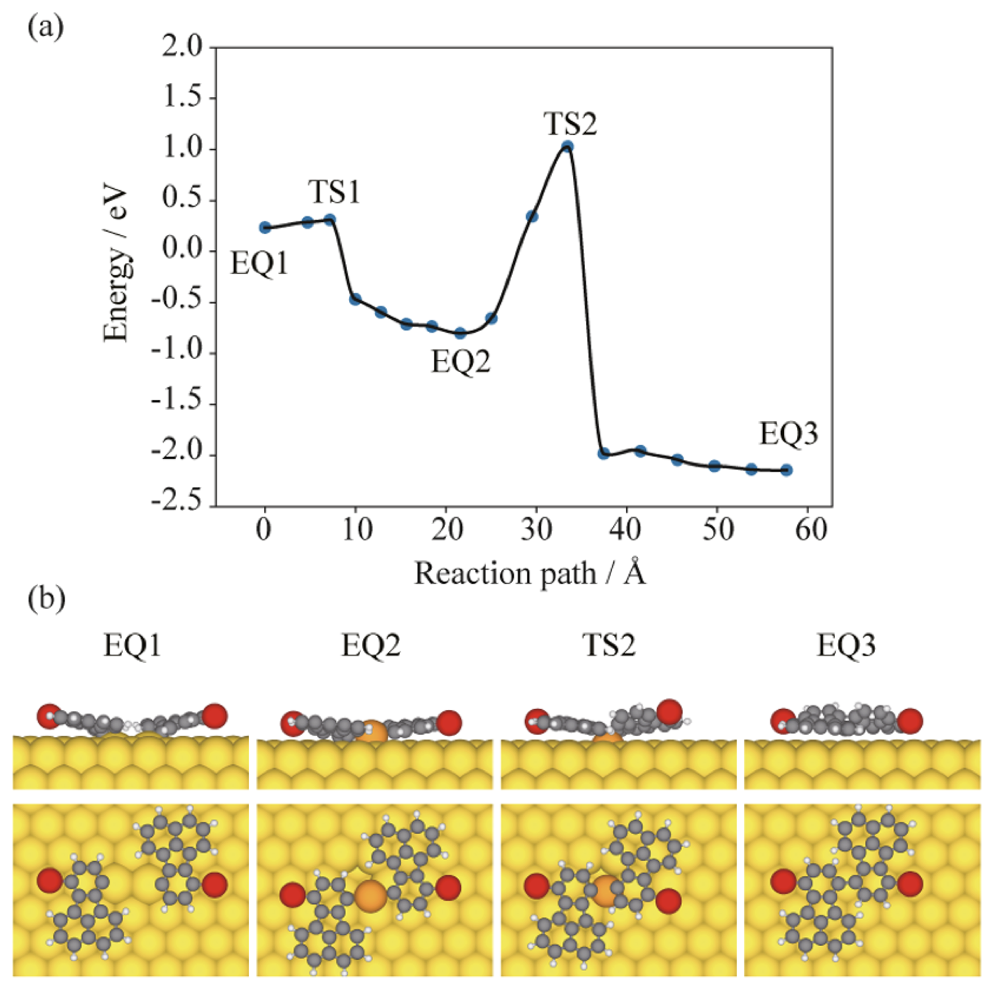
\includegraphics[width=0.75\columnwidth]{Fig/adatominformation.png}
\caption{(a) Energy profile of the coupling reaction of bromofluoranthene radicals through an organometallic intermediate along the reaction path. The horizontal axis indicates the distance between neighboring images. The energy is shown with respect to that of an isolated radical on the surface. (b) Top and side views of the initial (EQ1), transition (TS1, TS), intermediate (EQ2), and final (EQ3) geometries. Adapted from Ref.~\cite{jpcc2018}}
\label{fig:7}
\end{figure}

\subsection{Objectives}

{\comm RZK0426: I will write this section after the main results are discussed.}

{\comm RZK0426: This text is moved from the adatom intro because it reads as conclusions, not intro.} 

{\color{blue} Thus, it can be naturally derived that there is a competition between ideal-surface atoms and adatoms which actually take part in the structure of intermediates in Ullmann coupling. Also if it is ideal-surface atoms that comprise intermediates, these ideal-surface atoms can also be fully extracted out from the first layer and become extracted adatoms, which can be regarded as an approach to create adatoms on metal surface.}

{\lock

The focus of this work is on the role of adatoms in the surface Ullmann reaction, exemplified by the coupling of two phenyl rings -- one of the most studied and simple model of the Ullmann process.

Can the coupling be effectively catalyzed by an adatom, extracted or pre-existing? Is the energy of the reaction sufficient to create an adatom and whether there are any barriers along the extraction pathway?

Limitation: Aryl=Phenyl. Cu(111) only. Three halogens. How to limit the literature review?

%RZZK: as well as the microscopic mechanisms of interaction of all species with various defects, energy profile

{\comm RZK0426: Any remarks on what can be learnt from further studies of the mechanism? Ask Dima.}

}


\section{Methods}
%\subsection{Computation Models}

\subsection{Computational details}
{\color{blue}
The periodic density functional theory calculations were performed using the Perdew–Burke-Ernzerhof (PBE) for the exchange-correlation functional, the projector augmented wave method for the ion-core electron interactions, and a plane-wave basis set as implemented in the Vienna ab-initio simulation package (VASP) code. Van der Waals (vdW) interactions were included using the DFT-D3 method to describe the nonlocal correlation energy. All relaxations were performed with applying spin-polarization.

All Cu(111) surfaces were
modeled by four-layer slab consisting of 192 Cu atoms and at least \SI{15}{\angstrom} of vacuum. Each layer is made up with 48 (p(8 $\times$ 6)) Cu atoms. The energy cut-off for the plane-wave basis was set to \SI{800}{\electronvolt} and a $3\times 3 \times1$ k-mesh was adopted. The mesh density of k points was kept fixed in related calculations with primitive cells. All atoms were fully relaxed until the MAX force on the atom was less than 0.02 \si{\electronvolt}$/$\si{\angstrom}$^{2}$. 

Transition-state calculations were carried out using a Climbing-Image Nudged Elastic Band (CI-NEB) and Dimer methods with VTST code\cite{ullmann_59}. An improved initial guess~\cite{ullmann_60, ullmann_99} for minimum energy path was conducted in CI-NEB calculation, different number of intermediates were interpolated between the initial and final configurations due to the total distance among all atoms. Plus, All atoms were fully relaxed until the MAX force on the atom was less than \SI{0.1}{\electronvolt}/\si{\angstrom}$^{2}$ in CI-NEB calculations.

Generally the value of most thermodynamic functions can be derived from our DFT optimization results. 
{\comm ZZ: Need more details about the math derivation, added later
}


Monomers of surface Ullmann coupling reaction include chlorobenzene, bromobenzene and iodobenzene. We explored the mechanism of each elementary step.
%In the dehalogenation step, the CI-NEB method was used to the effect of chlorine, bromine and iodine on dissociation of carbon-halogen bonds. 
%Later in formation of phenyl--Cu--phenyl and C--C bond step, 
%Choice for the zero-energy state.
Clean, ideal Cu(111) surface with a halobenzene in gas phase (not adsorbed) is chosen to be zero-energy state in the energy profile (Fig.~\ref{fig:completeenergy}), other intermediates are present with relative values.
}
\section{Results and Discussion}

RZK0422: Re-read several times, make corrections, make sure it is clear to a reader new to the field. Polish English. Present data clearly.

\subsection{Physisorption}

{\color{blue}
Organic precursors will be adsorbed on metal surface before undergoing chemical transformations. 
The data in Table.~\ref{table:bondlength} indicate the interaction between organic molecules and metal surface are mainly physisorption. Compared with previous work using optB86b exchange-correlation functional, the trend and magnitude of growth from bromobenzene to iodobenzene are extremely similar. The strong binding of halobenzene is primarily due to the interaction of $\pi$-system and halogen with metal surface. The chemisorption energy of Br$_2$ molecule on Cu(111) is \SI{4.08}{\electronvolt}.
%The adsorption energies calculated in this work for a single molecule of chlorobenzene, bromobenzene and iodobenzene on Cu(111) are \SI{-1.06}{\electronvolt}, \SI{-1.18}{\electronvolt} and \SI{-1.37}{\electronvolt}, respectively (notated as \textbf{PHYS} in Fig.~\ref{fig:completeenergy}). 
%The predicted binding interaction is slightly stronger than the ones obtained previously using optB86b exchange-correlation functional: \SI{-0.95}{\electronvolt} for bromobenzene and \SI{-1.12}{\electronvolt} for iodobenzene~\cite{jacs2013}. It is worthy to mention that the difference in the strength of binding between iodobenzene and bromobenzene on Cu(111) is almost the same in our and previous works.

%RZK0415: The strong binding between the surface and halogenated benzenes is primarily due to the interaction of (a) the $\pi$-system (b) halogen and . For example, the energy of interaction between biphenyl and the metal is ZZZ whereas Br$_2$ molecule interacts with the surface by ZZZ.

%RZK0422: The following text is not mine and should not be in the red zone. My comment above is only a template, not the final text. Either (a) or (b) should be chosen in the final text. Moreover, 4.08 eV seems to be too strong for a vdW interaction.


}

% \begin{table*}
% \centering
% \begin{tabular}{ lcccc  }
%  \hline
%  \hline
%  Property & Chlorobenzene & Bromobenzene & Iodobenzene & Biphenyl \\ 
%  \hline 
%  {E (\si{\electronvolt}) } & 1.06 & 1.18 & 1.37 & 1.72\\ 
%  \hline
%  {E${\rm_{ref}}$ (\si{\electronvolt})~\cite{jacs2013}} &  & 0.95 & 1.12 & \\ 
%  \hline
%  \hline
% \end{tabular}
% \caption{Adsorption energy of multiple molecules on Cu(111)}
% \label{table:physisorbtion}
% \end{table*}

\begin{figure*}[hbt]
\centering
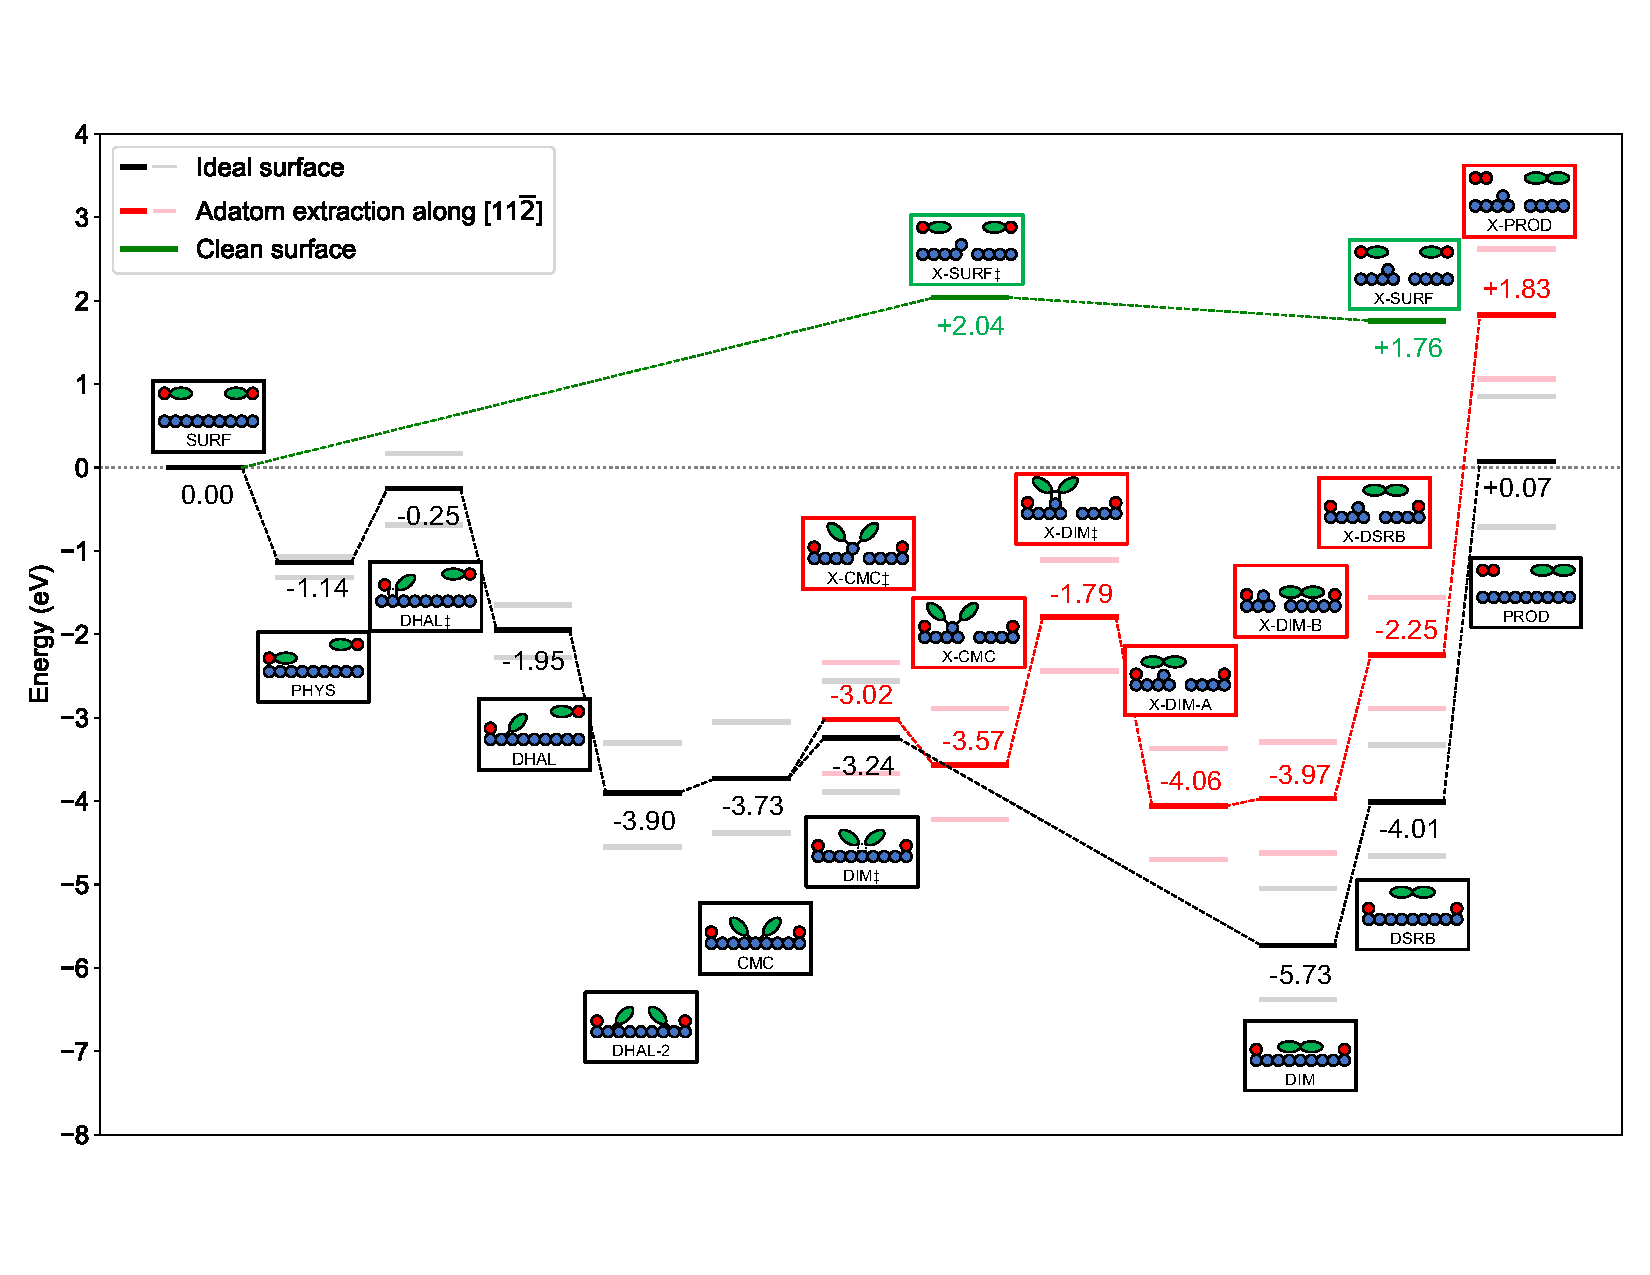
\includegraphics[width=1.\textwidth]{Fig/main-profile.pdf}
\caption{Energy profile of the Ullmann coupling of monohalogentated benzenes on the Cu(111) surface. In the schematic labels, blue and red circles denote copper and halogen atoms, respectively, whereas green ovals denote phenyl groups. Levels shown with bright colors are states with bromine as the halogen, whereas the faint upper and lower levels denote states with chlorine and iodine as the halogen, respectively. RZK0422: Rename the final SURF state to PROD and re-calculate its energy as the sum of: gas-phase Br2 molecule, gas-phase biphenyl, and pure surface. Same for the red pathway: X-PROD.}
\label{fig:completeenergy}
%\label{fig:Clfinal}
\end{figure*}

\subsection{Dehalogenation}

%RZK0312: Put Figures~\ref{fig:dissociation_Cl}, \ref{fig:dissociation_Br} and \ref{fig:dissociation_I} into supplementary information (SI). Keep only the structures (not the energy profile) for bromobenzene in the main text. Learn how to make references to a different document in LaTeX and make references to the figures in the SI.
%Note that these figures are of low quality. Atoms are pixilated -- higher resolution in VMD is necessary. Ball-and-stick is a poor choice to show alongated bonds in transition states. Graphs are poorly formatted (as discussed today). For all figures that remain in the main text much better formatting is necessary. Please look at figures in other articles (for example atoms in figure~\ref{fig:7}
%c) and make ours of the same quality. 

%RZK0317: Too many numbers in the text are difficult to read. Energies and energy barriers for all steps can be easier to compare if they are shown in a table or a figure (discussion is needed). Table might show, for each elementary step, energy of the forward reaction and it energy barrier. This data can also be shown in the figure, if halogens are kept separate.

%RZK0317: Energy profiles for all three halogens (or even five halogen-metal combinations) must be presented in the same plot (details to be discussed).

\begin{figure*}[hbt]
\centering
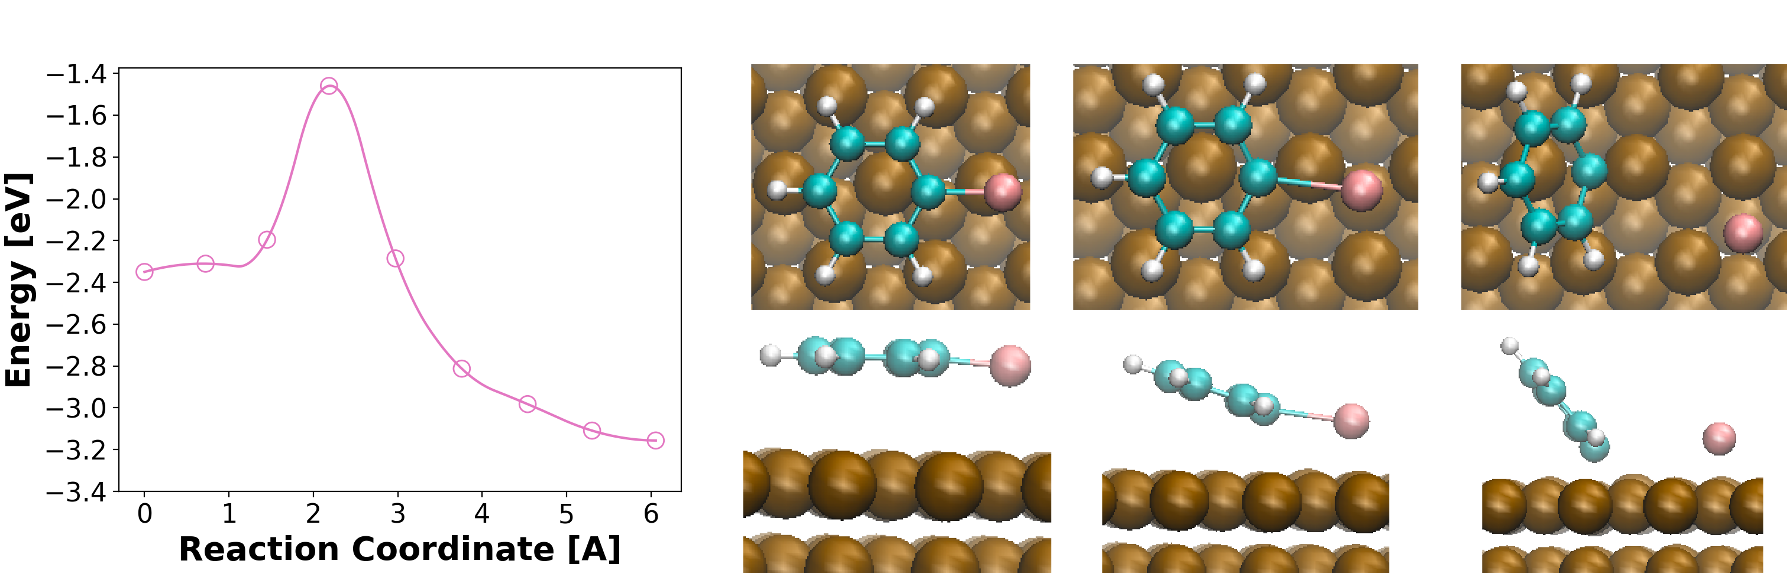
\includegraphics[width=1.0\textwidth]{Fig/dissociation_Br.pdf}
\caption{Dissociation of the C--Br bond on the Cu(111) surface. Yellow, cyan, white, red, RYK spheres represent copper, carbon, hydrogen, bromine, RYK atoms, respectively. 
%RZK0326: All figures with atoms need further work. The sideways view is not necessary here because it does not provide any useful info. Hydrogen and carbon spheres must be visible. Copper spheres are way too small: your choice of Cu radius makes Cu metal look like a layered material. The resolution of spheres is terrible -- they do not look like sphere but more as polygons. There should be no lines on sphere surfaces. If in doubt about the choice of parameters, see Fig.~\ref{fig:7} as an example of an excellent figure. In addition to this, all your figures and graphs have inappropriately low resolution. Do not use raster figures for your images, use vector formats: eps or pdf (zoom in Fig.~\ref{fig:completeenergy} to see how great vector format looks like.). If you cannot print a true vector figure, increase the resolution of all raster figures to at least 600 dpi. Journals do not accept anything raster images with the resolution lower than 300 dpi.
%RZK0415: I am not sure about the relevance of the NEB profiles in the figures. If we never discuss the shapes of the profiles then we should report only energies of the initial, transition and product states. If only the three states are reported on the energy profile, then it is NOT necessary to repeat data from the main energy figure.
%RZK0415: The energy profile mostly duplicates the main figure. I suppose it should be moved to SI. Without the energy graph the figure fits into one column. The top-view figure contains edge effects, which is highly undesirable. The side-view does not need four layers. All states should be labeled in the corner of the slab.
}
\label{fig:dissociation_Br}
\end{figure*}

{\lock

Fig.~\ref{fig:dissociation_Br} shows the structures of the initial, transition and final states (labeled as \textbf{PHYS}, \textbf{DHAL$\ddagger$} and \textbf{DHAL} in Fig.~\ref{fig:completeenergy}) for the debromination of the physisorbed bromobenzene on Cu(111). Dechlorination and deiodination have similar energy and geometry change trend (see \sinfo for the figures of dechlorination and deiodination).

}{\color{blue}

%[RZK0317: The logic of the paragraph below is not clear]

%Our results show that energy change of the dehalogenation step are \SI{-0.58}{\electronvolt}, \SI{-0.81}{\electronvolt} and \SI{-0.96}{\electronvolt} for chlorobenzene, bromobenzene and iodobenzene, respectively. It indicates that dehalogenation reactions on the copper surface are all exothermic. 
Our results show that dehalogenation reactions on the Cu(111) are all exothermic(Table.~\ref{table:bondlength}), rather than highly endothermic in gas phase~\cite{jacs2013}, verifying the catalysis role of copper surface in this step.
The energy barriers decrease in the order of chlorobenzene $>$ bromobenzene $>$ iodobenzene, in agreement with the corresponding experimentally measured temperatures required to complete dehalogenation on Cu(111) (Table.\ref{table:exp-temp}). This trend of different halogens is also consistent with the reported dissociation results of 1,4-dihalobenzene on Cu(110)\cite{ullmann_52}, illustrating that iodoaryl derivatives are the most reactive species in copper-confined ullmann coupling while chloroaryls are the least ones. It should be noted that this step has been investigated previously~\cite{jacs2013} with identical molecular orientation of species on surface using optB86b XC-functional (data listed in Table~\ref{table:bondlength}). The trend and magnitude of vary in energy change and barrier for different halogens are consistent with our conclusion, which is supported by Bell-Evans-Polanyi principle. The slight difference in the energy value can be interpreted by different functional usage and size of slab model for computation.

{\comm ZZ will add details how the XC-functional influence the calculation (overestimate/underestimate) later.}

\sout{The energy barrier of the dehalogenation on surface decreases from chlorobenzene} (\SI{1.24}{\electronvolt}) \sout{to bromobenzene} (\SI{0.89}{\electronvolt}) \sout{and to iodobenzene} (\SI{0.63}{\electronvolt}). \sout{This trend is in agreement with the trend of experimentally measured temperatures required to complete dehalogenation. On Cu(111), iodobenzene has been observed to dissociate at} \SI{175}{\kelvin}~\cite{ullmann_87}, \sout{while bromobenzene dissociates at} \SI{160}{\kelvin}~\cite{ullmann_67}. \sout{There is no data referred to dehalogenation temperature of chlorobenzene, but it can be inferred from the existing data of dihalogenated precursors that chlorobenzene dissociates at significantly higher temperature than bromobenzene and iodobenzene.}

\sout{Previous DFT calculation has demonstrated that the free energy barrier of nucleophilic substitution of chlorobenzene and bromobenzene with hydride in solution are} \SI{1.11}{\electronvolt} and \SI{1.01}{\electronvolt}~\cite{ullmann_86}. 


%RZK0317: Bell-Evans-Polanyi principle? (ZZ: added)



%RZK0317: Any comments? (ZZ: added)
%RZK0415: Did they study the same orientation of the molecule? (ZZ: yes, almost the same)

}

\begin{table*}
\centering
\begin{tabular}{ lcccccc  }
 \hline
 \hline
 Distance & Halogen & \textbf{PHYS} & Increase & \textbf{DHAL$\ddagger$} & \textbf{DHAL} & Change \\ 
 \hline 
 \multirow{3}{*}{C--Hal (\si{\angstrom})} & Cl & 1.74 & +0.44 & 2.18 & 3.99 & +2.25\\ 
 %\cline{2-5}
 & Br & 1.91 & +0.55 & 2.46 & 4.10 &+2.19 \\ 
 %\cline{2-5}
 & I & 2.12 & +0.49 & 2.61 & 5.10 &+2.98 \\ 
 %\cline{2-5}
 \hline
 \multirow{3}{*}{C--Cu (\si{\angstrom}) } & Cl & 3.54 & -1.02 & 2.52 & 2.01 & -1.53\\ 
 & Br & 3.40 & -0.63 & 2.77 & 2.01 & -1.39\\ 
 & I &3.42 &-0.69 & 2.73 & 2.01 & -1.41\\ 
 \hline
 \multirow{3}{*}{Hal--Cu (\si{\angstrom}) } & Cl & 2.99 & -0.62 & 2.37 & 3.50 & +0.51\\ 
 & Br & 2.89 & -0.49 & 2.50 & 3.57 & +0.68\\ 
 & I &2.80 &-0.16 & 2.64& 3.74 & +0.94\\ 
 \hline
 \hline
 Energy & & & Barrier & & & Change \\
 \hline
 \multirow{3}{*}{E (\si{\electronvolt}) } & Cl & -1.07 & 1.24 (+0.35) &0.17 &-1.65 & -0.58 (+0.23)\\ 
 & Br &-1.14 & 0.89 &-0.25 & -1.95& -0.81\\ 
 & I  & -1.32 & 0.63 (-0.26) & -0.69& -2.28& -0.96 (-0.15) \\ 
 \hline
 \multirow{2}{*}{E (\si{\electronvolt})~\cite{jacs2013}} & Br &-0.95 & 0.66 & & & -0.68 \\ 
 & I & -1.12& 0.40 (-0.26) & & & -0.81 (-0.12) \\ 
 \hline
 \hline
\end{tabular}
\caption{Geometric and energetic characterization of the dehalogenation step. Energies are reported relative to the \textbf{SURF} state. Values in parentheses are properties relative to those of bromine-containing states. Energetic data in reference is calibrated with the same zero-energy state in this work.}
%RZZK: Consider adding comparison to Br to all properties in parenthesis, as show in several examples: property(Hal) - property(Br).
\label{table:bondlength}
\end{table*}

{\color{blue}

%RZK0317: In the paragraph below, more numerical data must be presented in a Table and less in the text. Text should discuss main trends. (ZZ: added table)

Selected geometric parameters of the intermediates have also been summarized in Table~\ref{table:bondlength}. \sout{the distances between carbon and halogen which are going to dissociate a covalent bond, the angle of phenyl ring with respect to surface have both suffered successively changes.} In \textbf{PHYS} of halobenzene, the distance between carbon and halogen is consistent with the calculated C--halogen covalent bond length (\SI{1.76}{\angstrom} in chlorobenzene, \SI{1.91}{\angstrom} in bromobenzene and \SI{2.14}{\angstrom} in iodobenzene) in gas phase based on B3LYP functional DFT calculations. These distances show a continued growth till \textbf{DHAL} states, and dissociated halogen atoms all occupy the hollow site on Cu(111) surface in the end of dehalogenation. Interestingly, C--halogen distances in three different \textbf{DHAL$\ddagger$} transition states show consistent approximately \SI{0.5}{\angstrom} longer than corresponding C--halogen lengths in \textbf{PHYS} , suggesting that different dehalogenation reactions on Cu(111) follow similar mechanisms.

The angle of phenyl rings also suffer successively changes, parallel in \textbf{PHYS}, tilt in the process of dehalogenation and finalize with an apparent slope in \textbf{DHAL}. The interaction between unsaturated carbon and copper atom shortens their distance to same \SI{2.01}{\angstrom} in three different \textbf{DHAL} states, and these copper atoms are all raised approximately by \SI{0.12}{\angstrom} from their original positions.
The same C--Cu distances in \textbf{DHAL} suggest that the dissociated halogen atoms have little effect on the interaction of unsaturated carbon and copper atoms. However, halogen atoms have obvious influence on dissociated phenyl ring, resulting in their different tilt angles, deiodinated phenyl ring is inclined around \SI{70}{\degree} to metal surface, larger than debrominated and dechlorinated phenyl rings both at around \SI{50}{\degree}.

}

{\comm RZK0317: Discuss the role of adatoms in the dehalogenation step. Our results and/or old results can be discussed. Old results can be discussed briefly since they are already presented in the introduction. }

%RZK0422: Do not capitalize all words in titles, including section titles. Capitalize only the first word.

{\color{blue}

It has been proposed that the adatom could be extracted out to become an adatom in dehalogenation step. The energy of the adatom formation during the dehalogenation step can be compared to the high \SI{1.76}{\electronvolt} energy of the adatom extraction on the clean metal surface (Fig.~\ref{fig:completeenergy}, RYK-green pathway). The extraction on the clean surface has higher activation energy of \SI{2.04}{\electronvolt} than the approximately \SIrange{0.88}{0.96}{\electronvolt} of extraction with dehalogenation simultaneously due to previous work\cite{chemeurope2017}. It can be concluded that extracting an metal atom out to create an adatom require much less energy compared to creating it on clean surface. It can be noted that the activation energy of dehalogenation without adatom extraction is \SI{0.89}{\electronvolt}, similar to with adatom extraction. At the same temperature, dehalogenation with and without adatom formation should occur simultaneously on Cu(111) surface.



Summarizing the data of the first step, Cu(111) surface has been proven to evidently reduce the energy barrier of the dehalogenation of chlorobenzene, bromobenzene and iodobenzene. The copper surface can not only serve as a template and support for Ullmann coupling reaction, but also optimize the temperature condition for it to initialize. On Cu(111), the dehalogenation of iodobenzene is the most energetically favourable and chlorobenzene is the least. The mechanisms of three different halogens dissociation are very similar according to the angles and distance change in related species. And dehalogenation step is highly likely to create an adatom on Cu(111) surface.

}
%R1111: Do you mean our calculated enthalpies or experimental values? (%ZZ: add descriptions)
%R1111: Why your state lalbels (IM2, IM1) disagree with those in the final energy profile?(%ZZ: changed)
%R1111: Physisorption must be described before dissociation. Negative, not positive adsorption energies must be used
%In IM1, the precursor molecule was physisorbed by the surface, the adsorption energy are 1.06 eV, 1.18 eV and 1.37 eV, respectively for chlorobenzene, bromobenzene and iodobenzene. (%ZZ: added)
%
%R1111: Report bond elongations, not only bond lengths.
%R1111: Compare you results to Ph-I in barton2017fromation (Figure5-Cu_IS in their article). They do not have vertical position for the phenyl.  (%ZZ: recalculated, not vertical)
%R1111: Do we want to perform additional calculations to figure out the reason? Perhaps not now. (%ZZ: agree)

%R1111: The first sentence is trivial and must be removed. Do not define energy barrier in Results section. This definition is trivial and can be omitted.
%R1111: Some of these findings have been reported in the literature before. Comparison to previous calculations is necessary. "Trends are the same but numbers differ. Why? Do they use the same XC functional, basis set?" (%ZZ: added)


\subsection{Formation of C--Cu--C bridge intermediates}

{\color{blue}

As the data in Table.~\ref{table:idealsurface} shows, formation of C--Cu--C bridge intermediate (\textbf{CMC}) from two dehalogenated phenyl radicals (\textbf{DHAL-2}) is endothermic. Experimentally, dehalogenation and this step occur at same temperature (Table.~\ref{table:exp-temp}), corresponding to the relatively small energy change of this step in calculation. Gold surface is an exception that C--Au--C intermediates are rarely observed in experiment due to fast proceeding to coupling product after dehalogenation~\cite{ullmann_93, ullmann_100, ullmann_101, ullmann_102, ullmann_103, jacs2011}.

Compared to raised by \SI{0.12}{\angstrom} in \textbf{DHAL-2}, the copper atom interacted with two phenyl radicals is lifted by \SI{0.53}{\angstrom} in \textbf{CMC}, indicating a much stronger extraction.

%\textbf{DHAL-2} used here is well matched to the experimental STM image shown in Fig.~\ref{fig:organ}, the dissociated bromine atoms sit around in the formation of phenyl--Cu--phenyl structures. 
%The distance between two carbon atoms in the C--Cu--C bridge is \SI{3.10}{\angstrom}, which is \SI{1.61}{\angstrom} longer than the length of the connecting C--C in biphenyl. The angle of two phenyl rings connected to the Cu atom with respect to the surface are both \SI{52}{\degree}, this angle is the same as the tilt of a single phenyl in DHAL (\SI{52}{\degree}).

This step was reported to be exothermic in previous work\cite{pccp2010}. Two dehalogenated phenyl radicals are infinitely far this time, while they interact with adjacent copper atoms in previous work. The unignorable repulsion between result in a higher energy initial configuration and lead to the inconsistency.

%Formation of C--Cu--C bridge intermediate has been proven to play a significant role in the creation of adatom in surface Ullmann coupling. The interaction is potentially sufficient to extract an ideal surface copper atom out.

}

{\comm RZK0426: The result reported in pccp2010 for ideal-surface step is very different from our results. In their article this step is exothermic. This needs to be mentioned and perhaps discussed extensively. (ZZ: added)}

\begin{table*}
\centering
\begin{tabular}{ lccccccccc  }
 \hline
 \hline
 Distance & Halogen & \textbf{DHAL-2} & \textbf{CMC} & Increase & \textbf{DIM$\ddagger$} & \textbf{DIM} & Change & \textbf{DSRB} & \textbf{D-SURF}\\ 
 \hline 
 \multirow{3}{*}{C--C (\si{\angstrom})} & Cl & \multirow{3}{*}{$\infty$} & \multirow{3}{*}{3.10} & \multirow{3}{*}{-0.82} & \multirow{3}{*}{2.28} & \multirow{3}{*}{1.49} & \multirow{3}{*}{-1.61} & \multirow{3}{*}{1.49} &\multirow{3}{*}{1.49}\\ 
 & Br & &  &  &  & & & &\\ 
 & I & &  &  &  & & & &\\ 
 \hline
 \multirow{3}{*}{C--Cu (\si{\angstrom}) } & Cl & 2.01 & \multirow{3}{*}{2.06} & \multirow{3}{*}{-0.03} & \multirow{3}{*}{2.03} & \multirow{3}{*}{3.22} & \multirow{3}{*}{+1.16} & \multirow{3}{*}{} &\multirow{3}{*}{}\\ 
 & Br & 2.03 &  &  &  & & & &\\ 
 & I &2.02 &  &  &  & & & &\\ 
 \hline
 \multirow{3}{*}{Cu$_{\rm lift}$ (\si{\angstrom}) } & Cl & 0.12 & \multirow{3}{*}{0.53} & \multirow{3}{*}{-0.04} & \multirow{3}{*}{0.49} & \multirow{3}{*}{0.00} & \multirow{3}{*}{-0.53} & \multirow{3}{*}{0.00} &\multirow{3}{*}{0.00}\\ 
 & Br & 0.14 &  &  &  & & & &\\ 
 & I &0.12 &  &  &  & & & &\\ 
 \hline
 \hline
 Energy & & & (form \textbf{CMC}) & Barrier & & & Change & &\\
 \hline
 \multirow{3}{*}{E (\si{\electronvolt}) } & Cl & -3.30 & -3.05(+0.25) &+0.49 &-2.56 & -5.05 & -2.00& -3.33&0.85\\ 
 & Br &-3.90 & -3.73(+0.17) &+0.49 & -3.24& -5.73 & -2.00& -4.01&0.07\\ 
 & I  & -4.55 & -4.38(+0.17) & +0.49& -3.89& -6.38 & -2.00& -4.66&-0.71\\ 
 \hline
 \hline
\end{tabular}
\caption{Geometric and energetic characterization of the formation of C--Cu--C intermediate and C--C coupling step on ideal surface. Energies are reported relative to the \textbf{SURF} state. \textbf{DHAL-2} is twice the value as \textbf{DHAL} to simulate two infinite far dehalogenated phenyl radicals on Cu(111), \textbf{DSRB} with desorption of diphenyl product and \textbf{D-SURF} with further desorption of halogen atoms. Formation energy of \textbf{CMC} from \textbf{DHAL-2} should be same for different halogens, the differences here(in parenthesis) originate from the interaction between adjacent dissociated halogen atoms and organic fragments in \textbf{DHAL-2} in included.}
\label{table:idealsurface}
\end{table*}

\subsection{Formation of the C--C bond}

{\color{blue}
%In the final step of the Ullmann coupling a C--C bond is formed between two phenyl radicals. 
Two pathways of constructing C--C bond are investigated, the catalyzed Cu atom (1) returns to its original position with formation of biphenyl, metal surface retains defect-free, named \textit{ideal surface} path; (2) is fully extracted, creating an adatom-vacancy pair, adatam is free to diffuse after Ullmann reaction, named \textit{create adatom}
%The two pathways are discussed separately.
}

\subsubsection{Ideal surface}

{\lock

The energy profile of the first pathway is shown by the RYK-black line in Fig.~\ref{fig:completeenergy} whereas the details of NEB calculations are present in Fig.~\ref{fig:bondformlift}. The initial, transition and final states of this step are denoted as \textbf{CMC}, \textbf{DIM$\ddagger$} and \textbf{DIM}, respectively.

}{\color{blue}
 
%RZK0324: Do not use E_{barrier}. Write "the energy barrier" instead. 
%RZK0324: It would be better to use "the energy change" instead of $\Delta E$ but sometimes it is ok to use $\Delta E$ to shorten long sentences. 
%RZK0324: Replace all labels with the new ones. 
The energy change and barrier for this step are \SI{-2.00}{\electronvolt} and \SI{0.49}{\electronvolt}, respectively. These values are the same for all halogens because the initial and final modeling states do not contain halogen atoms in calculations. 
This step has also been investigated previously, energy change and barrier are provided as \SI{-1.90}{\electronvolt} and \SI{0.38}{\electronvolt} based on a smaller slab and same PBE exchange-correlation functional~\cite{pccp2010}, another work has reported \SI{-1.96}{\electronvolt} and \SI{0.14}{\electronvolt} for energy change and barrier respectively with a smaller slab as well and different optB86b exchange-correlation functional~\cite{jacs2013}.
%ZZ: more detailed analysis will be added.

Experiments have shown that the onset temperature for the final C--C bond-formation step is approximately \SI{300}{\kelvin}~\cite{sur_sci01} for synthesizing biphenyl on Cu(111) surface, which is in line with the calculated energy barrier (\SI{0.49}{\electronvolt}). In addition, this step is highly exothermic based on the \SI{-2.00}{\electronvolt} of energy barrier, and the final biphenyl product on Cu(111) possesses the lowest thermodynamic energy in Fig.~\ref{fig:completeenergy}. In experiment, surface Ullmann coupling of bromobenzene will proceed to biphenyl and two bromine atoms adsorbed on Cu(111) at \SI{350}{\kelvin}\cite{ullmann_67}, which agrees that biphenyl is the most thermodynamic stable species on coupling condition. Significantly higher temperature will end to the desorption of coupling product, even halogen atoms from metal surface.
{\comm RZK0324: Details on the agreement with experiment? (ZZ: added)}
 
Besides, Cu atom involved in C--Cu--C bridge structure is back to the first layer from \SI{0.56}{\angstrom} height in this step. The distance between two unsaturated carbon atoms starts from \SI{3.10}{\angstrom}, then shortened by \SI{0.82}{\angstrom} in the transition state and finalize at \SI{1.49}{\angstrom}, which is the same as the connecting C--C bond length in biphenyl molecule. The change of this distance is consistent with earlier work~\cite{sur_sci01}. The tilt angle of phenyl ring with respect to copper surface varied from \SI{52}{\degree} to \SI{34}{\degree} and ends in nearly \SI{0}{\degree}.
}

%R1111: LATER. We need to develop better notation for all chemical species and refer to them consistently.

%R1111: LATER. It is important to discuss the zero-energy for this step. Would it be more informative to use a common zero from the entire energy profile?
\begin{figure*}[hbt]
\centering
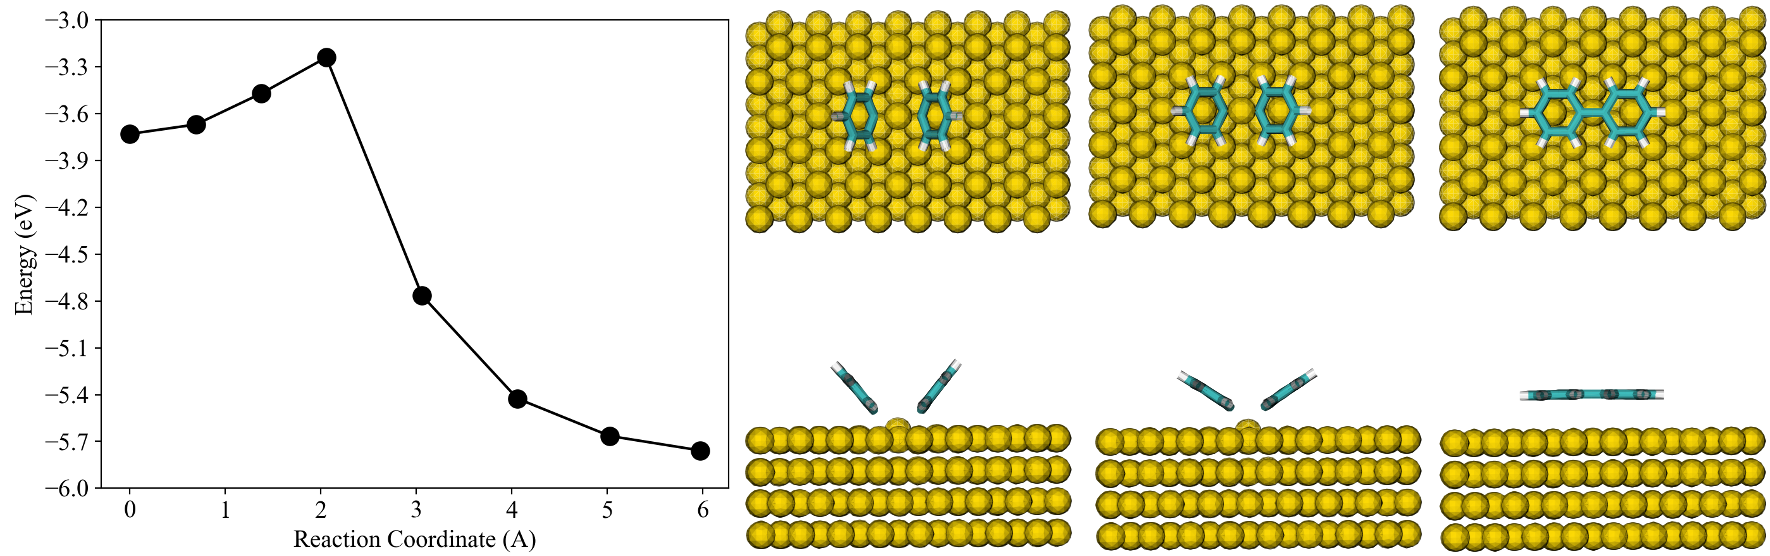
\includegraphics[width=1.0\textwidth]{Fig/bondformlift.pdf}
\caption{C-C bond formation with the copper atom returning to its original position. Left diagram is CI-NEB calculation, right part is the top and side view of \textbf{CMC}, \textbf{DIM$\ddagger$} and \textbf{DIM} in Fig.~\ref{fig:completeenergy}. RZK0324: The initial energy is that of the \textbf{CMC} state with bromine as the halogen.}
\label{fig:bondformlift}
\end{figure*}

\subsubsection{Create adatom}

\begin{table*}
\centering
\begin{tabular}{ lccccccccccc  }
 \hline
 \hline
 Distance & Halogen & \textbf{CMC} & Increase & \textbf{X-CMC$\ddagger$} & \textbf{X-CMC}(Change) & Increase & \textbf{X-DIM$\ddagger$} & \textbf{X-DIM-A}(Change) & \textbf{X-DIM-B}  \\ 
 \hline 
 \multirow{3}{*}{C--C (\si{\angstrom})} & Cl & \multirow{3}{*}{$\infty$} & \multirow{3}{*}{3.10} & \multirow{3}{*}{+0.45} & \multirow{3}{*}{3.89(+0.79)} & \multirow{3}{*}{-1.36} & \multirow{3}{*}{2.53} & \multirow{3}{*}{1.50(+2.39)} &\multirow{3}{*}{1.50}\\ 
 & Br & &  &  &  & & & & \\ 
 & I & &  &  &  & & & & \\ 
 \hline
 \multirow{3}{*}{C--Cu (\si{\angstrom}) } & Cl & \multirow{3}{*}{2.06} & \multirow{3}{*}{-0.26} & \multirow{3}{*}{1.85} & \multirow{3}{*}{1.96(-0.10)} & \multirow{3}{*}{-0.06} & \multirow{3}{*}{1.90} & \multirow{3}{*}{2.14(+0.18)} &\multirow{3}{*}{} \\ 
 & Br &  &  &  &  & & & &\\ 
 & I & &  &  &  & & & & \\ 
 \hline
 \multirow{3}{*}{Cu$_{\rm lift}$ (\si{\angstrom}) } & Cl & \multirow{3}{*}{0.53} & \multirow{3}{*}{+1.26} & \multirow{3}{*}{1.79} & \multirow{3}{*}{2.08(+1.55)} & \multirow{3}{*}{-0.20} & \multirow{3}{*}{1.88} & \multirow{3}{*}{1.87(-0.21)} &\multirow{3}{*}{0.00}\\ 
 & Br &  &  &  &  & & & &  \\ 
 & I & &  &  &  & & & & \\ 
 \hline
 \hline
 Energy  & & & Barrier & & & Barrier & & & \\
 \hline
 \multirow{3}{*}{E (\si{\electronvolt}) } & Cl & -3.05 & +1.38 &-1.67 &-3.26(-0.21) & -2.01 & -1.25& -3.42(-0.16)&-3.29\\ 
 & Br &-3.73 &+1.38 &-2.35 & -3.94(-0.21)& -2.01 & -1.93& -4.11(-0.16)&-3.97 \\ 
 & I  & -4.38 & +1.38 & -3.00& -4.59(-0.21)& -2.01 & -2.58& -4.76(-0.16)&-4.62\\ 
 \hline
 \hline
\end{tabular}
\caption{Geometric and energetic characterization of the C--C coupling step with creation of an adatom. Energies are reported relative to the \textbf{SURF} state.}
\label{table:adatom}
\end{table*}

{\lock

The energy profile of this pathway that leads to the creation of an adatom during the C--C bond-formation step is shown by RYK-red line in Fig.~\ref{fig:completeenergy}. The path contains three elementary steps: the adatom extraction, C--C bond formation on the top of adatom, and diffusion of biphenyl away from newly generated adatom. The two intermediates in this three-step process are denoted as \textbf{X-CMC}, \textbf{X-DIM-A}, whereas the final product is labeled as \textbf{X-DIM-B}. The two transition states are denoted as \textbf{X-CMC$\ddagger$}, \textbf{X-DIM$\ddagger$}.

}{\color{blue}

Fig.~\ref{fig:bondformadatom} shows trajectory from \textbf{CMC} to the C--Cu--C bridge intermediate on top of a fully extracted Cu adatom (\textbf{X-CMC}), followed by formation of dimer on this newly formed adatom (\textbf{X-DIM-A}). In \textbf{X-CMC} and \textbf{X-DIM-A}, a vacancy is generated on the original location of newly formed adatom. 
In the first step, an Cu atom is fully extracted out in \textbf{X-CMC} bridge intermediate, energy change and barrier are \SI{-0.20}{\electronvolt} and \SI{1.38}{\electronvolt}. The distance between two carbons forming C--Cu--C bridge increases to \SI{3.89}{\angstrom} (in \textbf{X-CMC}) from \SI{3.10}{\angstrom} (iin \textbf{CMC}), and cuts down by \SI{0.34}{\angstrom} in \textbf{X-CMC$\ddagger$}. The tilt angle flattens to \SI{13}{\degree} from \SI{34}{\degree}.

%%% Late steps
%R1111: What effect is responsible for the energy lowering upon adatom creation in IM5? Note that for I--Ph on Cu the extraction+diffusion during the C-I breaking step produces the overall uphill step. PRIORITY1. Remove Ph in IM3, IM4, IM without geometry relaxation (only the metal surface, not phenyl).

In the second step of forming C--C bond with newly formed adatom, energy change and barrier are \SI{-0.17}{\electronvolt} and \SI{2.01}{\electronvolt}. It ends with the formation of a new covalent C--C with a bond length of \SI{1.50}{\angstrom}, the former distance between these two carbons is \SI{3.10}{\angstrom} in \textbf{X-CMC}, and is condensed by \SI{0.57}{\angstrom} in \textbf{X-DIM$\ddagger$}. The tilt angle in \textbf{X-DIM-A} is a little twisted to \SI{-9.1}{\degree}. The configuration of biphenyl should be a nearly plane structure, this can be explained by the fact that the newly formed C--C is directly on the top of fully extracted Cu adatom. The distance from the Cu adatom to formed C--C bond is \SI{1.66}{\angstrom}, leading to the repulsion force and distort the two phenyl ring to such a degree.
This path will finally reach the state where a new adatom, a vacancy spot and a biphenyl formed on copper surface. Ideally there are no interaction among these three species (\textbf{X-DIM-B}). The energy of \textbf{X-DIM-B} is increased by \SI{0.14}{\electronvolt} compared to \textbf{X-DIM-A}.

In addition to the mechanism describe above, we explored an alternative reaction pathway directly from \textbf{X-CMC} to \textbf{X-DIM-B} instead of passing \textbf{X-DIM-A}. In this path, the formation of C--C bond and the diffusion of newly formed adatom away take place simultaneously, rather than one after the other in former path. The CI-NEB data is geometry is shown in \sinfo. Since this path displays an exceedingly high activation energy around (\SI{3.0}{\electronvolt}), and surpassing the previous energy barrier (\SI{2.01}{\electronvolt}) to a large scale, it seems not plausible to occur actually in nature.

Besides, we also investigated the effect of Ullmann coupling intermediates on creation of adatoms, as shown in Fig.~\ref{fig:onlysurface}. The bottom line shows the potential energy of \textbf{DHAL-2}, \textbf{CMC} and \textbf{X-CMC} in Fig.~\ref{fig:completeenergy}. The surface configuration of these three intermediates are separated from the slab and perform a single point energy calculation, the results are displayed in the top line. The energy of copper surface is increased by \SI{1.48}{\electronvolt} from \textbf{CMC} to \textbf{X-CMC}, but the potential energy of \textbf{X-CMC} is \SI{0.20}{\electronvolt} lower than \textbf{CMC}, this means that the interaction between two phenyl species and the ideal surface Cu is strong to extract the Cu atom out of first layer, and even lead to a more stable state on potential energy surface.

}



\begin{figure}[hbt]
\centering
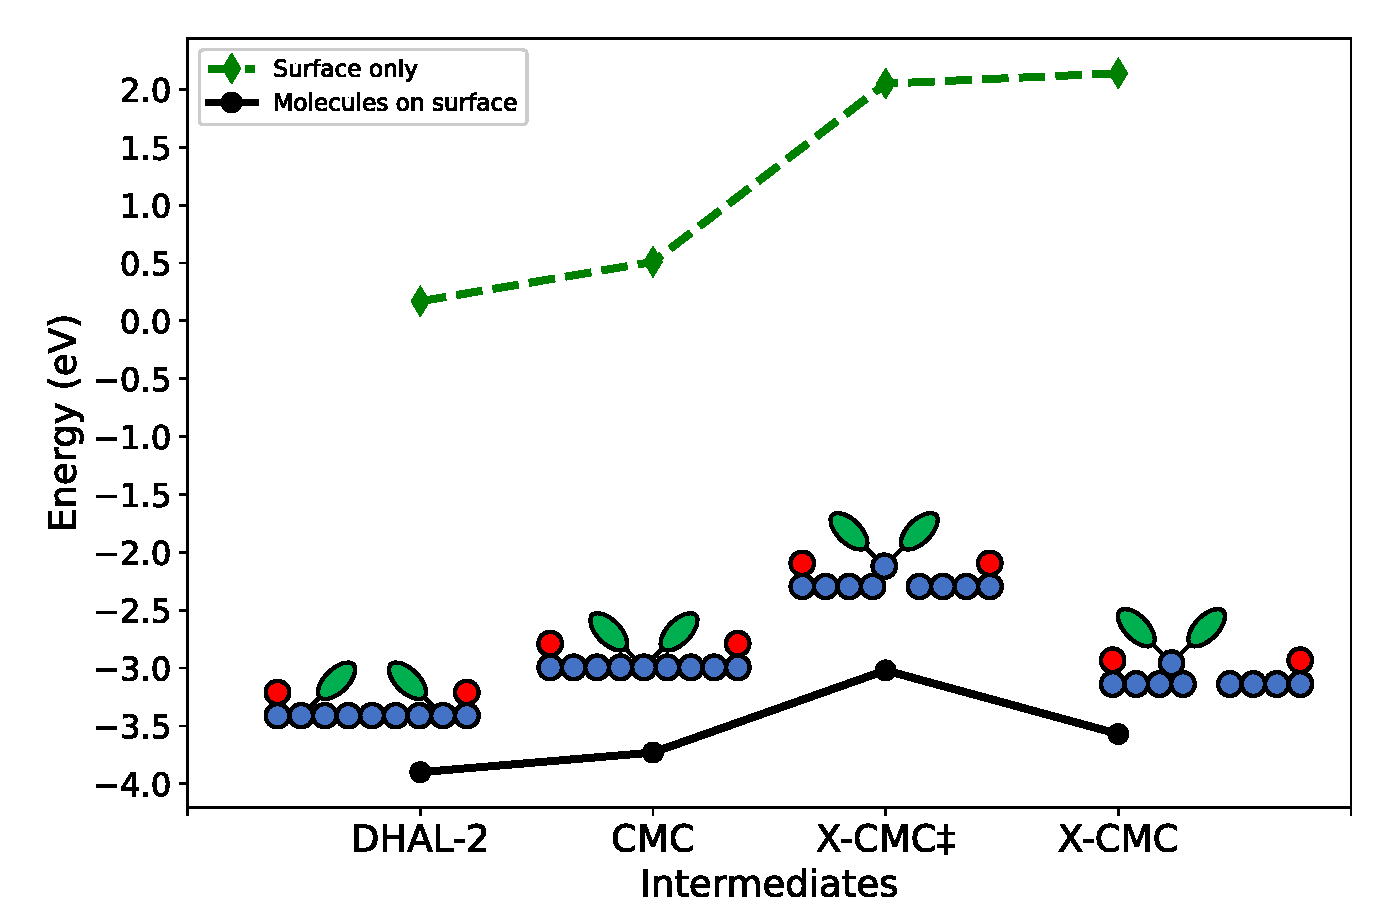
\includegraphics[width=0.45\textwidth]{Fig/onlysurface.pdf}
\caption{Energy diagram of \textbf{DHAL-2}, \textbf{CMC} and \textbf{X-CMC}, top line is the energy of pure Cu(111) surface geometry in \textbf{DHAL-2}, \textbf{CMC} and \textbf{X-CMC}, and the bottom line is the energy of Ullmann reaction species on surface.}
\label{fig:onlysurface}
\end{figure}


\begin{figure*}[hbt]
\centering
\includegraphics[width=1.0\textwidth]{Fig/adatom_extraction.pdf}
\caption{C-C bond formation through extraction of adatom in Path II. Left diagram is the energy of CI-NEB calculation, right part is the top and side view of \textbf{X-CMC}, \textbf{X-DIM$\ddagger$}, \textbf{X-CMC}, \textbf{X-DIM$\ddagger$}, and \textbf{X-DIM} in Fig.~\ref{fig:completeenergy}, sphere colors are set same as above.}
\label{fig:bondformadatom}
\end{figure*}

RZK0324: We need to decide whether to keep the 3 C--C bond formation NEB figures in the main text. It is definitely useful to keep those with the adatom. The three steps -- extraction, bond formation and diffusion -- should be combined into one. All NEB figures should be formatted in the same way as the dehalogenation step. 

RZK0324: Spin density maps of the adatom-containing intermediates.

%R1111: All titles and subtitles must use sentence case. It means that only the first word is capitalized. Do not capitalize all words!
\subsubsection{Ideal surface vs create adatom}

{\color{blue}
The possibility of two paths above are compared in multiple aspects.
The potential energy data and simplified cartoons geometry are present in Fig.~\ref{fig:completeenergy}. Two mechanism begin to vary from \textbf{CMC}, ideal surface path (black path) is both kinetically and thermodynamically more favourable due to a lower-energy transition state and more stable product. This suggests that at the same temperature condition, the reaction involved in ideal surface path will take place at a higher speed and account for a larger percentage. In experiment, phenyl radical species require temperature at \SI{350}{\kelvin} to accomplish C--C bonds on Cu(111) surface, this is more or less corresponding to a higher activation energy than \SI{0.49}{\electronvolt} obtained in ideal surface, this can be explained by the fact that all energy diagram are collected from potential energy, instead of free energy. Under a constant pressure, free activation energy will reflect authentic reaction condition. Taking the entropy contribution into consideration, the energy barrier should be larger, details will be discussed in entropy correction section.

In these two path, the final coupling steps seem similar from \textbf{X-CMC} to \textbf{X-DIM-A} and from \textbf{CMC} to \textbf{DIM}. The only difference is C--C forming on top an adatom in former path, and on ideal surface in latter path, though the energy barrier is highly distinct. This can be explained by the geometry of their entirely unequal transition state. 

However, the evidence in geometry provides a different result. In experiment, the distance between two carbons in C--Cu--C bridge structure is \SI{4.5}{\angstrom} \textpm\ \SI{0.6}{\angstrom} based on the STM image of this bridge intermediates. This corresponds to the distance in \textbf{X-CMC} of creation of an adatom path, which is \SI{3.89}{\angstrom}, but this distance in \textbf{CMC} is \SI{3.10}{\angstrom}. This means that the C--Cu--C intermediates is more likely to possess an adatom, this adatom is either from an ideal surface or it is an pre-existing adatom.

Taking the reaction condition into consideration. The temperature of final forming C--C bond from two phenyl species need to go up to above \SI{350}{\kelvin}~\cite{sur_sci01}. The activation energy of \textbf{CMC} evolved to \textbf{DIM$\ddagger$} in ideal surface path and to \textbf{X-CMC} in creation of an adatom path are \SI{0.38}{\electronvolt} and \SI{1.37}{\electronvolt}, respectively. The experimental temperature can meet the requirement of both two pathways, but the reaction in ideal surface path will occur with a higher speed.

RZK0422: The alternative transition states must be described. What is the energy barrier with the alternative TS compared to that with X-DIM-ddagger? 

}

%R1111: Compare C--C distance in IM4 and IM5 to the experimental data for Ph-Halogen. Can we see IM5 experimentally? 3.89Ang vs 3.1Ang. (%ZZ: Added)


%R1111: Note that the difference between dimer1 and dimer2 is smaller than the difference between FS1 and IS. Probably because the dimer interacts stronger with the adatom than with the surface. 


\subsection{Desorption of products}

{\color{blue}
The desorption of the reaction products have also been observed experimentally with temperature programmed desorption. Biphenyl has been reported to complete the desorpion on Cu(111) surface at \SIrange{400}{450}{\kelvin}\cite{ullmann_104}, which is nearly \SI{100}{\kelvin} higher than the coupling temperature.
The dissociated halogen atoms on surface will desorb even at much higher temperature. For instance, bromine atoms start to leave Cu(111) surface at \SI{900}{\kelvin} and higher, iodine atoms start at \SI{800}{\kelvin} \cite{jacs2013, ullmann_104}. 

Energy change of desorping formed biphenyl molecule is \SI{1.72}{\electronvolt}, and of desorping two chlorine atoms to chlorine gas molecule, two bromine atoms to bromine gas molecule and two iodine atoms to iodine gas molecule are \SI{4.18}{\electronvolt}, \SI{4.08}{\electronvolt} and \SI{3.95}{\electronvolt}, respectively. 
%RZK0422: As suggested before, calculate the energy of PROD state and report desorption energy of Halogen$_2$ molecule, not two separate atoms.
Desorping biphenyl molecule requires \SI{1.72}{\electronvolt} of energy, corresponding to increase the annealing temperature \SI{100}{\kelvin} higher than coupling temperature to remove biphenyl on Cu(111). 
And desorping bromine atoms require higher energy than iodine atoms, which is well matched to the higher temperature for bromine in experimental observation. 
Such a high desorption energy for halogen atoms becomes a nasty issue for practical surface Ullmann coupling. The dissociated halogen atoms will remain on metal surface and impede the further diffusion of chemical species for coupling. Removing the halogens can effectively optimize the speed and quality of synthesizing polymer structure in surface Ullmann coupling.
}



%%% Early steps
%R1111: LATER. Do we need adatom calculations for TS1? Perhaps only one or two halogen-metal pairs (for complete diagram). How will it affect the subsequent steps? Will the PH-Adatom roam the surface together before encountering the second Ph? PRIORITY6.

%R1111: Why there is no Cu-atom lifting during the C-X bond dissociation? Compare to previous works. Actually partial lifting is a process with a barrier for Au and Ag surfaces but not for Cu. We might need to reproduce this after all. --> More comparison to the existing calculation is required.

%RZK1222: This important effect needs to be properly described. The height of TS2-1 means that IM5, once formed will not undergo the C--C bond formation and can be viewed as an undesirable by-product of the reaction (unless it exists in quick equilibrium with IM4, which can be entropically hindered -- hard to find that vacancy again).

%RZK1222: How difficult is it to push the adatom (with attached organic radicals) DOWN?

\subsection{Coupling catalyzed by an existing adatom}
{\color{blue}
In addition to two paths discussed above in surface Ullmann coupling, we also consider the copper atom involved in surface Ullmann coupling is a pre-existing adatom on Cu(111). It is a superficial evaluation since in the calculations, a vacancy always exists next to the adatom, the interaction between the adatom and the vacancy has been ignored to presume an adatom has formed on Cu(111) before any surface Ullmann coupling precursors are adsorbed.

In the diagram, the initial state is the same as the one in Fig.~\ref{fig:completeenergy}. Overall the reaction is highly exothermic with a pre-existing adatom (from \textbf{X-SURF}). This adatom displays a high availability of interaction to various intermediate species in surface Ullmann coupling. Can an existing adatom revert back to its original ``clean'' form to catalyze another event? The answer to this question will provide the prediction on the sustained catalytic ability of pre-existing adatoms. However, it seems negative from our results. First, adatom-coordinated species cannot react with the sufficiently low barrier to produce weakly adsorbed products. Example: C--C bond formation is hindered by the high activation barrier. Second, adatom-coordinated species are anchored to the adatom can relocate inside a pre-existing vacancy at a defect site on surface and back to \textbf{CMC}, then complete the coupling reaction with the ideal surface path. Example: the activation barrier of reverse \textbf{CMC} to \textbf{X-CMC} is lower than C--C bond formation on top of an adatom.

It suggests that the reaction will be interrupted at C--Cu--C organometallic intermediate with a pre-existing adatom. Compared to forming C--C bond, it prefers to diffuse to nearby vacancy site, refill it and catalyze the final production synthesize.
}
{\comm back to reform the halogen bond will be discussed once the transition state is done}




\begin{figure*}[hbt]
\centering
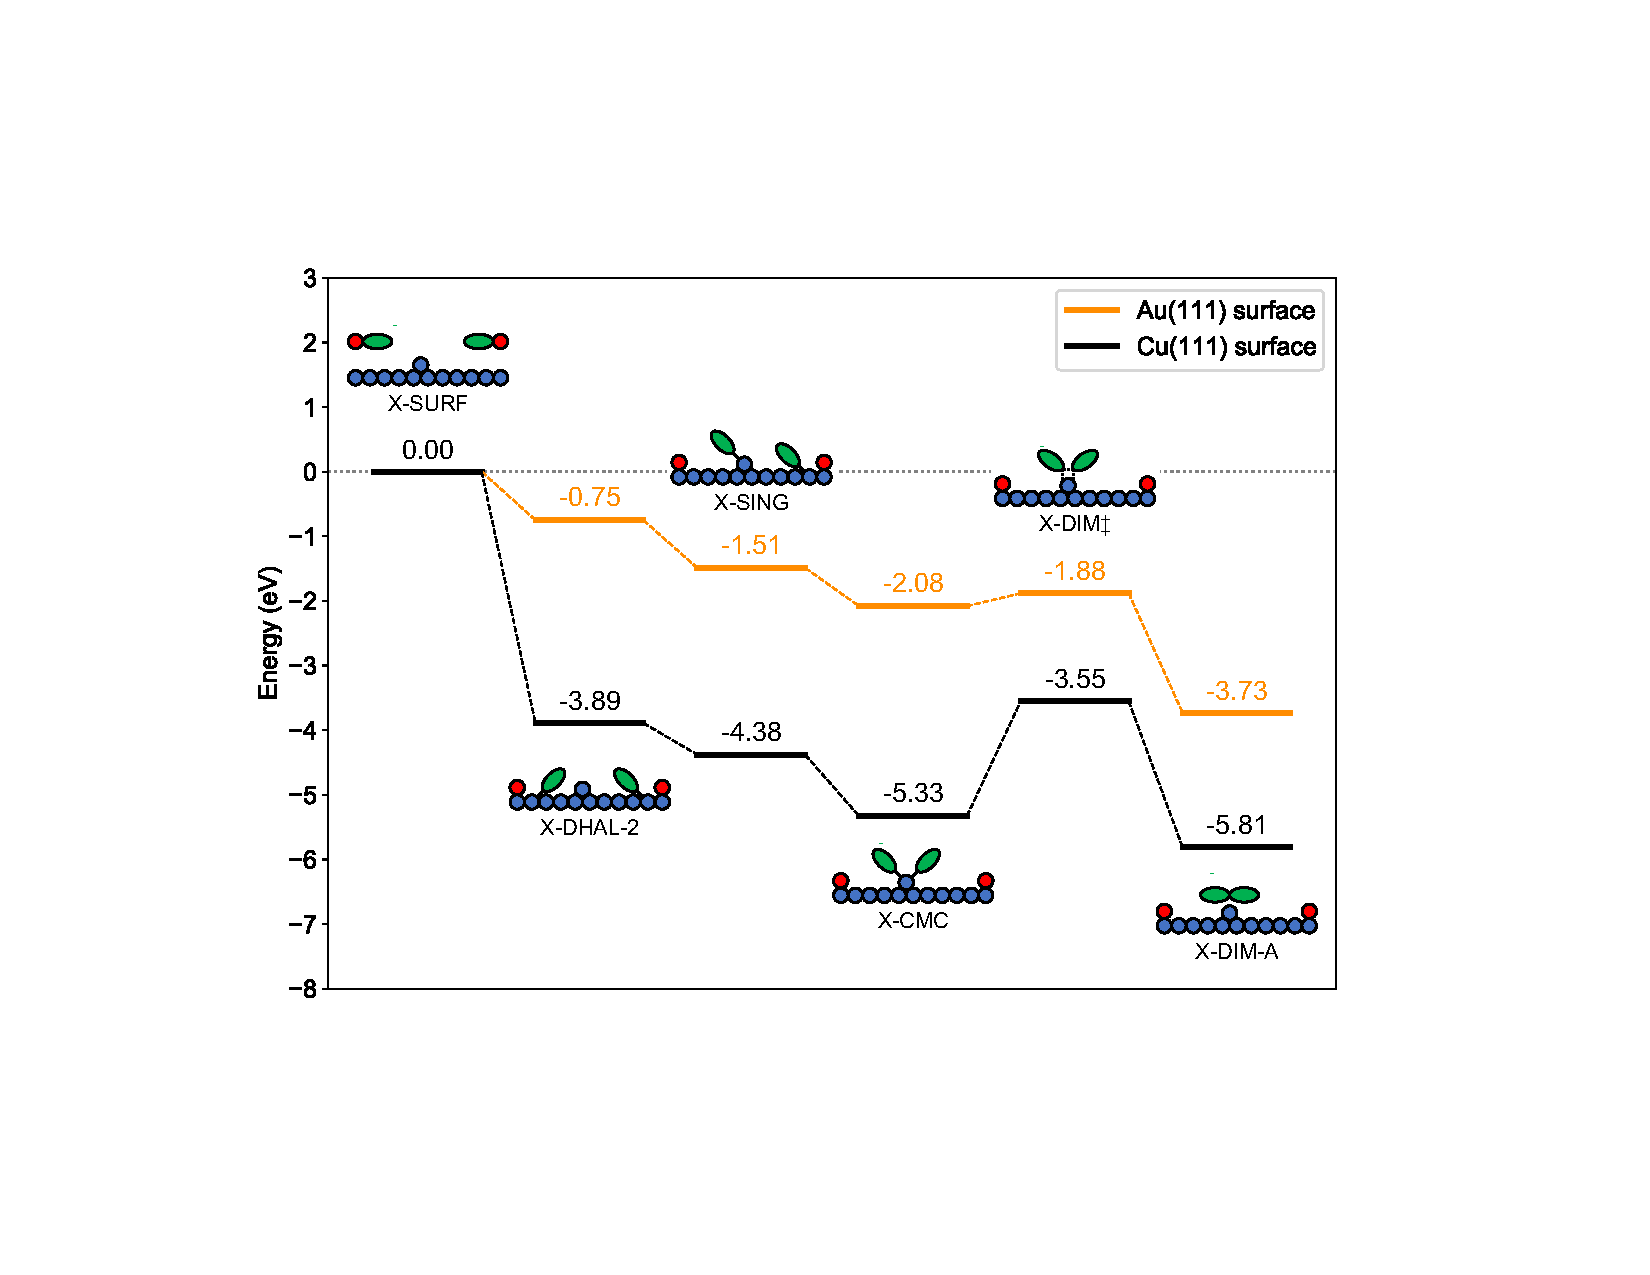
\includegraphics[width=0.98\textwidth]{Fig/ullmann_adatom.pdf}
\caption{The energy diagram of bromobenzene on Cu(111) surface Ullmann coupling reaction with a pre-existing adatom. (Scarlet circle represents bromine atom). ZZ: reformat this figure will be done in the future } 
\label{fig:adatomullmann}
\end{figure*}

{\comm (from Rustam)RZK0422: Can an existing adatom revert back to its original ``clean'' form to catalyze another event? It does not look plausible. First, adatom-coordinated species are anchored to the adatom too strongly to simply diffuse away. Examples. Second, adatom-coordinated species cannot react with the sufficiently low barrier to produce weakly adsorbed products. Example: C--C bond formation is hindered by the high activation barrier. C--Halogen bond formation? (ZZ: added in main text)}

\section{Entropy correction and free energy calculation}
{\color{blue}
An unignorable disagreement exits between the experimental data and our DFT results. The calculated energy barrier of dehalogenation is \SI{0.89}{\electronvolt} (\textbf{PHYS}-\textbf{DHAL$\ddagger$}), which is  higher than the energy barrier from two dehalogenated phenyls to the biphenyl (\textbf{DHAL-2}-\textbf{DIM$\ddagger$}). In experiment, the latter step always require a higher temperature to accomplish than dehalogenation step, which has been descried by the data in Table.~\ref{table:exp-temp}. This issue has also existed in other works~\cite{jacs2013, pccp2010}. We are considering this general discrepancy aroused from the ignorance of entropy in theoretical calculations. 

DFT calculations make a useful contribution to elucidating the mechanism behind the adsorption of molecules on surface, and allow precise prediction on energy and geometry. However, DFT calculations are basically limited to \SI{0}{\kelvin} temperature, describing potential energy and trend, instead of free energy change. Specifically in surface Ullmann coupling reaction, the formation of dimer consists of the combination of two dehalogenated species, which will lead to an effective decrease in entropy and make a non-negligible contribution to free energy change. Thus, to bridge the gap between experiments and simulation data in surface Ullmann coupling at finite temperature, entropy must be taken into consideration. 

Here the free energy diagram (Fig.\ref{fig:entropy}) is obtained after the entropy correction is done to our previous potential energy data. We treated three dimensional free gas molecules and two dimensional adsorbed species both with transnational motion exclusively, the temperature condition for all species are at \SI{200}{\kelvin} and \SI{400}{\kelvin}, respectively labeled in Fig.\ref{fig:entropy}, pressure of gas molecule is $10^{-10}$ mba, which is widely used ultra high vacuum condition in surface Ullmann coupling, and the concentration of adsorbed molecules is \SI{10e-16}{\per\metre\squared}, which is validated by STM image in Ref.~\cite{ullmann_67}. Details are discussed in \sinfo.

Zero energy state is fluctuated up in free energy due to including the entropy correction of gas bromobenzene. At \SI{400}{\kelvin}, the free energy barrier stay unchanged as \SI{0.89}{\electronvolt}, while the free energy barrier from \textbf{DHAL-2} to \textbf{DIM$\ddagger$} changes to \SI{1.09}{\electronvolt} from previous \SI{0.66}{\electronvolt}. The energy required for C--C coupling from two dehalogenated species has effectively increased in free energy calculations, which is further matched with the experimentally higher temperature in second step.

Our study suggests that the entropy contribution to free energy will affect the process of surface Ullmann coupling.The entropy calculation depends much on surface coverage, temperature and pressure, a highly consistent reaction condition parameter setup will allow more accurate results in DFT calculations. However, our model for two dimensional lattice adsorption is a superficial model, aimed at providing insight into narrowing the gap between theoretical calculation and experiment. 
}
\begin{figure*}[hbt]
\centering
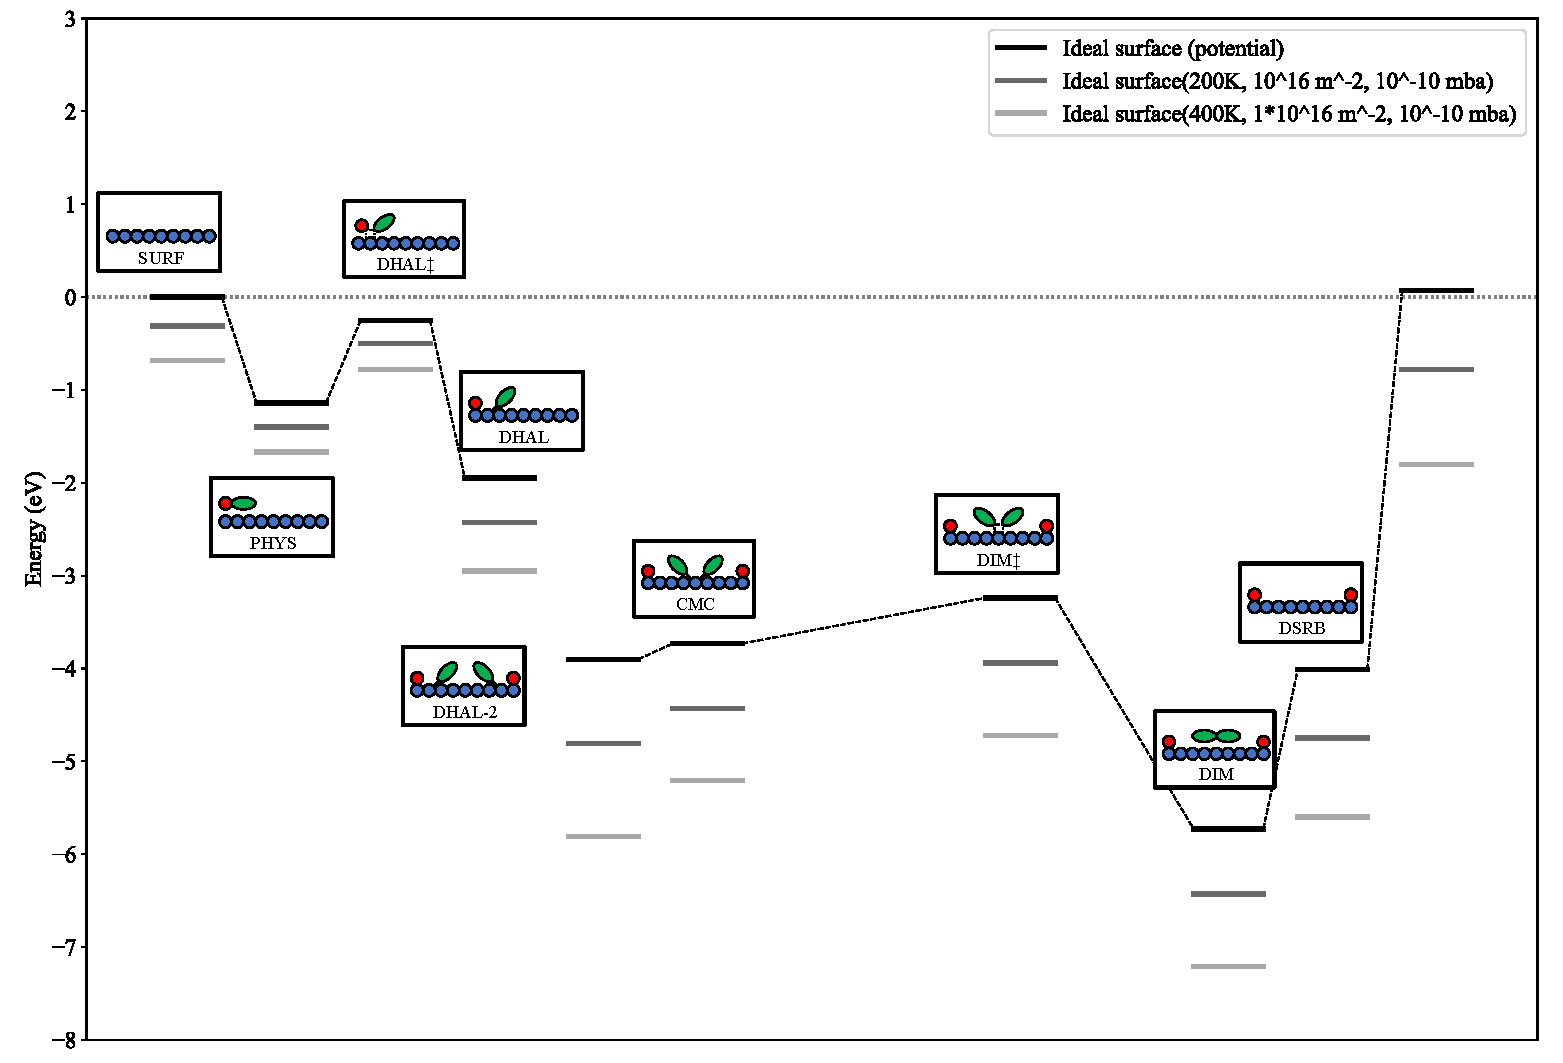
\includegraphics[width=0.98\textwidth]{Fig/entropy-correction.pdf}
\caption{The free energy diagram of bromobenzene on Cu(111) surface Ullmann coupling reaction without extraction of copper atom.}
\label{fig:entropy}
\end{figure*}


\section{Conclusions}
{\color{blue}
We have systematically studied the surface Ullmann coupling reaction of chlorobenzene, bromobenzene and iodobenzene on commonly employed Cu(111) surface with computation methods. Also the role of metal atom involved in each elementary step of forming biphenyl molecule are studied. Mainly the energy and molecular geometry of two different pathways: (1) a partially lifted up copper atom takes part in the formation of C--Cu--C bridge structure and back to it original position in first layer of surface with the construction of new C--C bond; (2) a copper atom and a vacancy is formed by fully extraction of C--Cu--C bridge structure, and a new adatom is created with forming C--C bond on copper surface are compared based on DFT calculation results. A simple discussion on the circumstance that an adatom exists before the surface Ullmann coupling occurs and interact with coupling-related species has also been constructed.

The effect of different halogens mostly agree with the results descried in previous works. It can be concluded that halogens will mainly influence the dehalogenation step and produce little effect on later steps. After forming C--Cu--C bridge intermediate structure, the path of partially lifting ideal surface atom is much more energetically favorable both in thermodynamics and kinetics, compared with the path of creating a new adatom. This suggests that Ullmann coupling on copper surface is more likely to occur through a non-adatom formation pathway, the metal atom will be partially lifted up while the C--Cu--C organometallic intermediates forms and back to its original position after completing the coupling reaction. However, it is also worthwhile to mention that the possibility that adatoms will take part in the Ullmann coupling process should not be ruled out. The heat released from the hehalogenation step is sufficient to compensate either C--C coupling through a non-adatom surface metal atom or through an adatom creating path. It means both of these two procedure can occur in nature but occupy different proportions and proceed in different velocity.

The path that adatom already exists from thermal fluctuation or defect before the coupling is roughly discussed. Pre-existing adatom can be regarded as a exceedingly plausible source for organometallic intermediates in surface Ullmann coupling on metal surface.
}
{\comm RZK: Clean adatoms can be created if the monomers interact strongly. Design?}

% \section{surface Ullmann coupling on other coinage surface}
We have also investigated surface Ullmann coupling of bromobenzene of Ag(111) and Au(111) surfaces other than Cu(111). Ag(111) and Au(111) are modeled in the same procedure as Cu(111), 4 layers (each layer contains 48 atoms) with 20 \SI{20}{\angstrom} slab is built and optimized.




\subsection{bromobenzene on Ag(111) surface}















\subsection{bromobenzene on Au(111) surface}

\section{acknowledgements}


\nocite{*}

\bibliographystyle{apsrev4-1} % Tell bibtex which bibliography style to use
\bibliography{references}% Produces the bibliography via BibTeX.

\end{document}








